\documentclass[
%% alle weiteren Papierformat einstellbar:
a4paper, %apaper,
%% keine Seitenzahlen:
%empty,
%% Schriftgröße (12pt, 11pt (Standard)):
11pt,
%% kleinere Überschriften:
%smallheadings,
%bibliography=totoc,
]
{scrartcl}

\input{packages.latex}

% chktex-file 18

\title{Spieltheorie}
\subtitle{Zusammenfassung}
\author{Martin Darmüntzel}

\begin{document}

\maketitle

\tableofcontents

\section{Die Nutzenfunktion}%
\label{sec:die_nutzenfunktion}

Eigenschaften der Konsummenge (\emph{consumption set}) $X$:
\begin{enumerate}
  \item $X \subseteq \RealNumbers^n_+$
  \item $X$ ist abgeschlossen ($\overline{X}$ ist offen)
  \item $X$ ist konvex
  \item $0 \in X$
\end{enumerate}

Es existiert die binäre Relation der Konsumentenpräferenz $\atleastasgood$ mit
$x_1 \atleastasgood x_2 \ \Leftrightarrow \ x_1$ ist mindestens genauso gut wie $x_2$.

\begin{axiom}[Vollständigkeit]
  \label{axiom:vollstaendigkeit}
  Für alle $x^1, x^2 \in X$ gilt entweder
  $x^1 \atleastasgood x^2$ oder $x^2 \atleastasgood x^1$.
\end{axiom}

\begin{axiom}[Transitivität]
  \label{axiom:transitivitaet}
  Für alle $x^1, x^2$ und $x^3 \in X$ gilt:
  wenn $x^1 \atleastasgood x^2$ und $x^2 \atleastasgood x^3$,
  dann gilt $x^1 \atleastasgood x^3$.
\end{axiom}

\begin{definition}[Präferenzrelation]
  Die binäre Relation $\atleastasgood$ auf der Konsummenge $X$ ist eine
  \emph{Präferenzrelation}, wenn es die Axiome~\ref{axiom:vollstaendigkeit}
  und~\ref{axiom:transitivitaet} erfüllt.
\end{definition}

\begin{definition}[strenge Präferenzrelation]
  Die binäre Relation $\strictlypreferredto$ auf der Konsummenge $X$ ist definiert als
  \begin{align*}
    x^1 \strictlypreferredto x^2
    \ \Leftrightarrow \
    x^1 \atleastasgood x^2 \text{ und } x^2 \notatleastasgood x^1
  \end{align*}
\end{definition}


Nutzen und Erwartungsnutzen

Siehe:
\begin{itemize}
  \item \href{https://de.wikipedia.org/wiki/Grenznutzen}{Grenznutzen}
  \item \href{https://de.wikipedia.org/wiki/Grenzrate_der_Substitution}{Grenzrate der
    Substitution}
\end{itemize}


\section{Statische Spiele mit vollständiger Information}%
\label{sec:statische_spiele_mit_vollstandiger_information}

\begin{definition}[Rationalität]
  Rational zu handeln bedeutet, dass ein Individuum aus einer Menge von Wahlmöglichkeiten
  eine Aktion $a$ so wählt, dass $a$ mindestens genauso gut wie jede andere Aktion $b$
  ist.
  Die Güte der Aktion ist durch die Nutzenfunktion bestimmt.
\end{definition}

\subsection{Strategische Spiele}%
\label{sub:strategische_spiele}

Ein Strategienprofil ist eine Funktion, die den Spielern bestimmte Aktionen zuweist.
Bei den Spielern $\{1,2,3\}$ und den Aktionsmengen
$A_1 = \{T, B\}, A_2 = \{L, R\}, A_3 = \{I, O\}$
ist bspw. $(a_1, a_2, a_3) = (T, L, O)$ ein Strategienprofil.
Eine besondere Notation ist die Variante $(b_i, a_{-i})$, welche bedeutet, dass Spieler
$i$ die Aktion $b_i$ und \emph{nicht} $a_i$ wählt.
Wenn $b_2 = R$ ist, dann ist $(b_2, a_{-2}) = (T, R, O)$.
Alles bleibt gleich, nur Spieler $2$ ändert die Aktion.

\begin{definition}[Strategisches Spiel mit ordinaler Präferenz]
  Ein strategisches Spiel (mit ordinaler Präferenz) besteht aus:
  \begin{itemize}
    \item einer Menge von Spielern $P = \{1, \ldots, n\}$
    \item für jeden Spieler: eine Menge von Aktionen $S_i$
    \item für jeden Spieler: Präferenzen über der Menge der Aktionsprofile
      $u_i: S_1 \times \ldots \times S_n \to \RealNumbers$
  \end{itemize}
\end{definition}

\subsection{Gefangendilemma}%
\label{sub:gefangendilemma}

Zwei Verdächtige werden verhaftet und angeklagt.
Die Polizei hat nicht genügend Beweise um beide zu verurteilen, es sei denn
einer von beiden gesteht.
Die Verdächtigen werden in verschiedene Zellen gesteckt und ihnen werden die
Konsequenzen der möglichen Aktionen erklärt.
Jeder kann entweder \emph{schweigen} (kooperieren) oder \emph{gestehen}
(defektieren, gegen den anderen aussagen) und jeder Gefangene möchte möglichst
wenige Jahre im Gefängnis verbringen.
Wenn beide schweigen, dann bekommt jeder 1 Jahr wegen kleinerer Delikte.
Wenn einer schweigt und der andere gesteht, dann wird der Geständige
freigelassen und der andere bekommt die Höchststrafe von 9 Jahren Haft.
Wenn beide gestehen bekommen beide durch die Zusammenarbeit mit der Polizei (das
Geständnis) nicht die Höchststrafe, sondern jeweils nur 6 Jahre ins Gefängnis.

Die Auszahlungsmatrix (Bimatrix) sieht wie folgt aus:
\begin{center}
  \begin{tabular}{cccc}
    & & \multicolumn{2}{c}{B}\\
    & & schweigt & gesteht\\
    \multirow{2}{*}{A} &
    schweigt & $-1, -1$ & $-9, \phantom{-}0$\\
    & gesteht & $\phantom{-}0, -9$ & $-6, -6$\\
  \end{tabular}
\end{center}

Die Ergebnisse haben besondere Namen:

\begin{table}[h]
  \centering
  \caption{Mögliche Erträge im Gefangenendilemma}
  \label{tab:moegliche_ertraege_im_gefangenendilemma}
  \begin{tabular}{ccr}
    \toprule
    \makecell{$T$\\ temptation\\ (Versuchung)} &
    \makecell{Verpfeifen, wenn der andere schweigt\\[1ex] (Defektion bei Kooperation)} &
    $0$\\
    \midrule
    \makecell{$R$\\ reward\\ (Belohnung)} &
    \makecell{Schweigen, wenn der andere schweigt\\[1ex] (Kooperation bei Kooperation)} &
    $-1$\\
    \midrule
    \makecell{$P$\\ punishment\\ (Bestrafung)} &
    \makecell{Verpfeifen, wenn der andere verpfeift\\[1ex] (Defektion bei Defektion)} &
    $-6$\\
    \midrule
    \makecell{$S$\\ sucker’s payoff\\ (Lohn des Gutgläubigen)} &
    \makecell{Schweigen, wenn der andere verpfeift\\[1ex] (Kooperation bei Defektion)} &
    $-9$\\
    \bottomrule
  \end{tabular}
\end{table}

Allgemein hat ein Gefangenendilemma folgende Struktur:
\begin{center}
  \begin{tabular}{cccc}
    & & \multicolumn{2}{c}{B}\\
    & & kooperiert & defektiert\\
    \multirow{2}{*}{A} &
    kooperiert & $R, R$ & $S, T$\\
    & defektiert & $T, S$ & $P, P$\\
  \end{tabular}
\end{center}
Dabei müssen diese Ungleichungen gelten:
\begin{align*}
  T > R > P > S \text{ und } 2R > T + S
\end{align*}
Die erste geht aus den einzelnen Präferenzen hervor und die zweite sorgt dafür, dass die
Verdächtigen sich bei Wiederholung nicht gegenseitig ausbeuten können.
Bei Wiederholung könnten sie abwechselnd kooperieren und defektieren und würden auf Dauer
mehr Nutzen haben.
Diese Möglichkeit muss ausgeschlossen werden.

\subsection{Bach oder Strawinski}%
\label{sub:bach_oder_strawinski}

Beim Gefangenendilemma ist das Hauptproblem, ob beide Spieler kooperieren.
Im folgenden Spiel sind sich beide einig, dass es besser ist zu kooperieren, aber sie sind
sich nicht über die Aktion einig.

Zwei Menschen wollen zusammen den Abend verbringen.
Zwei Konzerte stehen zur Verfügung: Bach oder Strawinski.
Eine Person präferiert Bach, die andere Strawinski.
Wenn sie auf verschiedene Konzerte gehen, sind sie beide gleich unglücklich, weil sie den
Abend nicht mit der anderen Person verbringen.
\begin{center}
  \begin{tabular}{cccc}
    & & \multicolumn{2}{c}{B}\\
    & & Bach & Strawinski\\
    \multirow{2}{*}{A} &
    Bach & $2, 1$ & $0, 0$\\
    & Strawinski & $0, 0$ & $1, 2$\\
  \end{tabular}
\end{center}

\subsection{Matching Pennies}%
\label{sub:matching_pennies}

Zwei Spieler wählen gleichzeitig ob sie Kopf oder Zahl einer Münze zeigen.
Wenn die Münzen die gleiche Seite zeigen, dann zahlt Spieler 2 einen Euro an Spieler 1.
Wenn sie verschiedene Seiten zeigen, dann zahlt Spieler 1 einen Euro an Spieler 2.

\begin{center}
  \begin{tabular}{cccc}
    & & \multicolumn{2}{c}{Spieler 2}\\
    & & Kopf & Zahl\\
    \multirow{2}{*}{Spieler 1} &
      Kopf & $\phantom{-}1, -1$ & $-1, \phantom{-}1$\\
    & Zahl & $-1, \phantom{-}1$ & $\phantom{-}1, -1$\\
  \end{tabular}
\end{center}

\subsection{Hirschjang (Stag hunt)}%
\label{sub:hirschjang_stag_hunt}

Eine Jägerin einer Gruppe hat zwei Optionen: entweder konzentriert sie sich auf die
Verfolgung eines Hirsches oder sie schießt vielleicht einen Hasen.
Wenn alle Jäger den Hirsch verfolgen, dann fangen sie ihn und teilen ihn gleich auf.
Wenn ein Jäger sich auf den Hasen konzentriert, dann entwischt der Hirsch und der Hase
gehört nur dem abtrünnigen Jäger.
Jeder Jäger präferiert einen Teil des Hirsches gegenüber einem Hasen.

Das Spiel besteht demnach aus den folgenden Elementen:
\begin{description}
  \item[Spieler] Die Jäger.
  \item[Aktionen] jeder Jäger hat die Aktionen $\{\emph{Hirsch}, \emph{Hase}\}$.
  \item[Präferenzen] Für jeden Jäger ist das Aktionsprofil $(\emph{Hirsch}, \ldots,
    \emph{Hirsch})$, also alle wählen Hirsch, am wertvollsten.
    Danach kommt für jeden Jäger das Profil, in dem er \emph{Hase} wählt, gefolgt von
    allen Profilen, in denen er \emph{Hirsch} wählt und irgendein anderer \emph{Hase}
    wählt (sodass er leer ausgeht).
\end{description}
Für zwei Spieler sieht das Spiel wie folgt aus:
\begin{center}
  \begin{tabular}{cccc}
    & & \multicolumn{2}{c}{Spieler 2}\\
    & & Hirsch & Hase\\
    \multirow{2}{*}{Spieler 1} &
      Hirsch & $2, 2$ & $0,1$\\
    & Hase   & $1, 0$ & $1,1$\\
  \end{tabular}
\end{center}

\subsection{Nash-Gleichgewicht}%
\label{sub:nash_gleichgewicht}

Ein Gleichgewicht ist eine stabile Situation, in der kein Spieler einen Anreiz hat, sein
Verhalten zu verändern.

Ein \emph{Nash-Gleichgewicht} ist ein Aktionsprofil $a^* = (a^*_1, \ldots, a^*_n)$,
bei dem kein Spieler $i$ eine bessere Aktion als $a^*_i$ wählen kann,
sofern die anderen Spieler $j$ an $a^*_j$ festhalten.

\begin{definition}[Nash-Gleichgewicht eines strategischen Spiels mit ordinaler Präferenz]
  Das Aktionsprofil $a^*$ ist genau dann ein Nash-Gleichgewicht,
  wenn es für jeden Spieler $i$ und für jede Aktion $a_i$ von Spieler $i$
  bezüglich der Präferenzen von $i$
  mindestens genauso gut wie das Aktionsprofil $(a_i, a^*_{-i})$ ist,
  bei dem Spieler $i$ die Aktion $a_i$ statt $a^*_{-i}$ wählt,
  während alle anderen Spieler $j$ jeweils $a^*_j$ wählen.

  Äquivalent gilt für jeden Spieler $i$
  \begin{align*}
    u_i(a^*) \geq u_i(a_i, a^*_{-i}) \quad \text{für jede Aktion $a_i$ von Spieler $i$.}
  \end{align*}
\end{definition}

\subsection{Beste-Antwort-Funktionen}%
\label{sub:beste_antwort_funktionen}

\begin{definition}[Beste-Antwort-Funktion]
  Die Menge der besten Aktionen von Spieler $i$ gegenüber den Aktionen $a_{-i}$ der
  anderen Spieler wird mit $B_i(a_{-i})$ notiert.
  Genau definiert wird sie als:
  \begin{align*}
    B_i(a_{-i}) & = \left\{
      a_i \in A_i :
      u_i(a_i, a_{-i}) \geq u_i(a'_i, a_{-i})
      \text{ für alle $a'_i \in A_i$}
    \right\}
  \end{align*}
  Jede Aktion in $B_i(a_{-i})$ ist mindestens so gut für Spieler $i$ wie jede andere
  Aktion von Spieler $i$, wenn die Aktionen der anderen Spieler $a_{-i}$ sind.

  Wenn jeder andere Spieler an der Aktion $a_{-i}$ festhält, dann kann Spieler $i$ nicht
  mehr erreichen, als durch eine Aktion aus $B_i(a_{-i})$.
\end{definition}

Im Spiel \emph{Bach oder Strawinski} ist
$B_1(\emph{Bach}) = \{ \emph{Bach} \}$ und
$B_1(\emph{Strawinski}) = \{ \emph{Strawinski} \}$.

Mit der Besten-Antwort-Funktion (auch Reaktionsfunktion genannt) lässt sich auch das
Nash-Gleichgewicht definieren:
das Aktionsprofil $a^*$ ist genau dann ein Nash-Gleichgewicht eines strategischen Spiels
mit ordinaler Präferenz, wenn jede Aktion der Spieler eine beste Antwort auf die Aktionen
der anderen Spieler ist:
\begin{align}
  \label{eq:beste_antwort_nash_gg}
  a^*_i \in B_i(a^*_{-i}) \text{ für alle Spieler $i$}
\end{align}
Wenn die Menge der besten Antworten aus genau einem Element besteht
($B_i(a_{-i}) = \{ b_i(a_{-i}) \}$),
dann wird dieses Element als $b_i(a_{-i})$ notiert.
Dann gilt:
\begin{align*}
  a^*_i = b_i(a^*_{-i}) \text{ für alle Spieler $i$}
\end{align*}

Mit der Beste-Antwort-Funktion lässt sich das Nash-Gleichgewicht finden.
Finde dazu die besten Antworten aller Spieler und finde dann die Aktionsprofile,
die~\ref{eq:beste_antwort_nash_gg} erfüllen.

\paragraph{Dominierte Aktionen}%
\label{par:dominierte_aktionen}

\begin{definition}[Strikte Domination]
  Eine Aktion $\hat{a}_i$ von Spieler $i$ wird \emph{strikt dominiert},
  wenn es eine andere Aktion $\tilde{a}_i \in A_i$ gibt,
  so dass $\tilde{a}_i$ zu einer strikt größeren Auszahlung führt als $\hat{a}_i$
  — unabhängig davon, welche Aktion von den Gegenspielern gewählt werden:
  \begin{align*}
    u_i(\hat{a}_i, a_{-i}) < u_i(\tilde{a}_i, a_{-i})
    \quad
    \forall a_{-i} \text{ der anderen Spieler}
  \end{align*}
\end{definition}

Im Gefangenendilemma wird \emph{Kooperieren} strikt von \emph{Defektieren} dominiert, weil
$T > R$ und $P > S$ gilt.

Es gilt Rationalität bei strikter Dominanz: ein rationaler Spieler wird niemals eine
strikt dominierte Strategie spielen.

\begin{definition}[Schwache Dominanz]
  Eine Aktion $\hat{a}_i$ von Spieler $i$ wird \emph{schwach dominiert}, wenn es eine
  andere Aktion $\tilde{a}_i \in A_i$ gibt, so dass gilt:
  \begin{align*}
    u_i(\hat{a}_i, a_{-i}) \leq u_i(\tilde{a}_i, a_{-i})
    \quad \forall a_{-i} \text{ der anderen Spieler}
  \end{align*}
  und
  \begin{align*}
    u_i(\hat{a}_i, a_{-i}) < u_i(\tilde{a}_i, a_{-i})
    \quad \text{für mindestens ein $a_{-i}$ der anderen Spieler}
  \end{align*}
\end{definition}

Ein rationaler Spieler kann durchaus eine schwach dominierte Strategie spielen.

\begin{definition}[dominante Strategie]
  Eine Strategie $s^*_i$ von Spieler $i$ ist eine \emph{strikt dominante} Strategie, falls
  sie alle anderen Strategien von Spieler $i$ strikt dominiert:
  \begin{align*}
    u_i(s^*_i, s) > u_i(s_i, s) \qquad
    \forall s_i \in S_i \setminus \{s^*_i\},
    \forall s \in S_{j \neq i}
  \end{align*}
\end{definition}

Wenn eine strikt dominante Strategie $s^*_i$ existiert, wird sie ein rationaler Spieler
immer wählen.

\begin{definition}[Iterative Eliminierung strikt dominierter Strategien]
  Wiederhole solange, bis sich nichts mehr ändert: finde eine dominante Strategie und
  eliminiere sie.
\end{definition}

Beispiel: 2 Spieler, 4 Strategien

\begin{center}
  \begin{tabular}{cccccc}
    & & \multicolumn{4}{c}{B}\\
    & & $b_1$ & $b_2$ & $b_3$ & $b_4$\\
    \multirow{4}{*}{A} & $a_1$ & $0,7$ & $2,5$ & $7,0$ & $0,1$\\
    & $a_2$ & $5,2$ & $3,3$ & $5,2$ & $0,1$\\
    & $a_3$ & $7,0$ & $2,5$ & $0,7$ & $0,1$\\
    & $a_4$ & $0,0$ & $0,-2$ & $0,0$ & $10,-3$\\
  \end{tabular}
\end{center}

Egal welche Strategie Spieler A wählt, für B ist $b_2$ immer besser als $b_4$, also wird
$b_4$ eliminiert:

\begin{center}
  \begin{tabular}{ccccc}
    & & \multicolumn{3}{c}{B}\\
    & & $b_1$ & $b_2$ & $b_3$\\
    \multirow{4}{*}{A} & $a_1$ & $0,7$ & $2,5$ & $7,0$\\
    & $a_2$ & $5,2$ & $3,3$ & $5,2$\\
    & $a_3$ & $7,0$ & $2,5$ & $0,7$\\
    & $a_4$ & $0,0$ & $0,-2$ & $0,0$\\
  \end{tabular}
\end{center}

Jetzt ist es egal, welche Strategie Spieler B wählt, für A ist $a_2$ immer besser als
$a_4$ und damit wird $a_4$ eliminiert:

\begin{center}
  \begin{tabular}{ccccc}
    & & \multicolumn{3}{c}{B}\\
    & & $b_1$ & $b_2$ & $b_3$\\
    \multirow{4}{*}{A} & $a_1$ & $0,7$ & $2,5$ & $7,0$\\
    & $a_2$ & $5,2$ & $3,3$ & $5,2$\\
    & $a_3$ & $7,0$ & $2,5$ & $0,7$\\
  \end{tabular}
\end{center}


\section{Dynamische Spiele mit vollständiger Information}%
\label{sec:dynamische_spiele_mit_vollstandiger_information}

\begin{definition}[Extensives Spiel mit perfekter Information]
  Ein extensives Spiel mit perfekter Information besteht aus
  \begin{itemize}
    \item einer Menge von \emph{Spielern}
    \item einer Menge von Folgen (\emph{terminalen Geschichten}) mit der Eigenschaft, dass
      keine Folge eine echte Teilgeschichte einer anderen Folge ist
    \item einer Funktion (der \emph{Spielerfunktion}), die einem Spieler jede echte
      Teilgeschichte irgendeiner terminalen Geschichte zuweist
    \item für jeden Spieler: Präferenzen über der Menge der terminalen Geschichten
  \end{itemize}
\end{definition}

\begin{definition}[Nash-Gleichgewicht eines extensiven Spiels mit perfekter Information]
  Das Strategieprofil $s^*$ in einem extensiven Spiel mit perfekter Information ist genau
  dann ein Nash-Gleichgewicht, wenn für jeden Spieler $i$ und jede Strategie $r_i$ von
  Spieler $i$ die von $s^*$ erzeugte terminale Geschichte $O(s^*)$ (abhängig von den
  Präferenzen von Spieler $i$) mindestens genauso gut ist, wie die von dem Strategieprofil
  $(r_i, s^*_{-i})$ erzeugte terminale Geschichte $O(r_i, s^*_{-i})$, in der $r_i$ von
  Spieler $i$ gewählt wurde, während jeder andere Spieler $j$ das Strategieprofil $s^*_j$
  gewählt hat.

  Äquivalent gilt für jeden Spieler $i$:
  \begin{align*}
    u_i(O(s^*)) \geq u_i(O(r_i, s^*_{-i})) \quad
      \text{für jede Strategie $r_i$ von Spieler $i$}
  \end{align*}
  wobei $u_i$ die Nutzenfunktion ist, die die Präferenzen von Spieler $i$ repräsentiert
  und $O$ die Auszahlungsfunktion des Spiels ist.
\end{definition}


\pagebreak

\section{Aufgaben}%
\label{sec:aufgaben}

\subsection{Serie 1}%
\label{sub:serie_1}


\subsection{Serie 2}%
\label{sub:serie_2}


\subsection{Serie 3}%
\label{sub:serie_3}

\paragraph{Aufgabe 1}%
\label{par:serie_3_aufgabe_1}

\begin{enumerate}
  \item Bestimmen Sie alle Nash-GG (in reinen Strategien) des folgenden Spiels in
    strategischer Form:
    \begin{center}
      \begin{tabular}{ccc}
        & $B$ & $S$\\
        \cmidrule{2-3}
        $B$ & $2,1$ & $0,0$\\
        \cmidrule{2-3}
        $S$ & $2,0$ & $1,2$\\
        \cmidrule{2-3}
      \end{tabular}
    \end{center}
  \item Bestimmen Sie alle Nash-GG (in reinen Strategien) des folgenden Spiels in
    strategischer Form in Abhängigkeit von $x$:
    \begin{center}
      \begin{tabular}{ccc}
        & $A$ & $B$\\
        \cmidrule{2-3}
        $U$ & $x,2$ & $2,0$\\
        \cmidrule{2-3}
        $D$ & $2,1$ & $4,2$\\
        \cmidrule{2-3}
      \end{tabular}
    \end{center}
  \item Bestimmen Sie alle Nash-GG (in reinen Strategien) des folgenden Spiels in
    strategischer Form:
    \begin{center}
      \begin{tabular}{ccc}
        & $L$ & $R$\\
        \cmidrule{2-3}
        $L$ & $-1, \phantom{-}1$ & $\phantom{-}1, -1$\\
        \cmidrule{2-3}
        $R$ & $\phantom{-}1, -1$ & $-1, \phantom{-}1$\\
        \cmidrule{2-3}
      \end{tabular}
    \end{center}
\end{enumerate}

\subparagraph{Lösung}%

\begin{enumerate}
  \item Die jeweils besten Antworten lauten:
    \begin{center}
      \begin{tabular}{ccc}
        & $B$ & $S$\\
        \cmidrule{2-3}
        $B$ & $\underline{2},\underline{1}$ & $0,0$\\
        \cmidrule{2-3}
        $S$ & $\underline{2},0$ & $\underline{1},\underline{2}$\\
        \cmidrule{2-3}
      \end{tabular}
    \end{center}
    Somit gilt $\text{NGG} = \{(B,B), (S,S)\}$.

  \item Unabhängig von $x$ sind folgende unterstrichenen Auszahlungen jeweils beste
    Antworten der Spieler:
    \begin{center}
      \begin{tabular}{ccc}
        & $A$ & $B$\\
        \cmidrule{2-3}
        $U$ & $x,\underline{2}$ & $2,0$\\
        \cmidrule{2-3}
        $D$ & $2,1$ & $\underline{4},\underline{2}$\\
        \cmidrule{2-3}
      \end{tabular}
    \end{center}
    Damit ist $(D,B)$ immer ein Element des NGG.

    Für die vollständige Bestimmung der Nash-Gleichgewichte bedarf es einer
    Fallunterscheidung von $x$ im Vergleich zur alternativen Auszahlung von $2$ für
    $(D,A)$.

    \begin{description}
      \item[$x<2$:] Die besten Antworten lauten:
        \begin{center}
          \begin{tabular}{ccc}
            & $A$ & $B$\\
            \cmidrule{2-3}
            $U$ & $x,\underline{2}$ & $2,0$\\
            \cmidrule{2-3}
            $D$ & $\underline{2},1$ & $\underline{4},\underline{2}$\\
            \cmidrule{2-3}
          \end{tabular}
        \end{center}
        Damit gilt: $\text{NGG} = \{(D,B)\}$.

      \item[$x=2$:] Die besten Antworten lauten:
        \begin{center}
          \begin{tabular}{ccc}
            & $A$ & $B$\\
            \cmidrule{2-3}
            $U$ & $\underline{x},\underline{2}$ & $2,0$\\
            \cmidrule{2-3}
            $D$ & $\underline{2},1$ & $\underline{4},\underline{2}$\\
            \cmidrule{2-3}
          \end{tabular}
        \end{center}
        Damit gilt: $\text{NGG} = \{(U, A), (D,B)\}$.

      \item[$x>2$:] Die besten Antworten lauten:
        \begin{center}
          \begin{tabular}{ccc}
            & $A$ & $B$\\
            \cmidrule{2-3}
            $U$ & $\underline{x},\underline{2}$ & $2,0$\\
            \cmidrule{2-3}
            $D$ & $2,1$ & $\underline{4},\underline{2}$\\
            \cmidrule{2-3}
          \end{tabular}
        \end{center}
        Damit gilt wie im Fall $x=2$: $\text{NGG} = \{(U, A), (D,B)\}$.
    \end{description}

  \item Die jeweils besten Antworten lauten:
    \begin{center}
      \begin{tabular}{ccc}
        & $L$ & $R$\\
        \cmidrule{2-3}
        $L$ & $-1, \phantom{-}\underline{1}$ & $\phantom{-}\underline{1}, -1$\\
        \cmidrule{2-3}
        $R$ & $\phantom{-}\underline{1}, -1$ & $-1, \phantom{-}\underline{1}$\\
        \cmidrule{2-3}
      \end{tabular}
    \end{center}

    Damit ist keine Strategiekombination Teil des Nash-Gleichgewichts und es gilt
    $\text{NGG} = \emptyset$.
\end{enumerate}

\paragraph{Aufgabe 2}%
\label{par:serie_3_aufgabe_2}

Bestimmen Sie für folgendes Spiel in Normalform alle Nash-Gleichgewichte in reinen
Strategien:

\begin{center}
  \begin{tabular}{ccccc}
    & & \multicolumn{3}{c}{Spieler 2}\\
    & & $L$ & $C$ & $R$\\
    \cmidrule{3-5}
    \multirow{3}{*}{Spieler 1}
    & $T$ & $0,1$ & $9,0$ & $2,3$\\
    \cmidrule{3-5}
    & $M$ & $5,9$ & $7,3$ & $1,7$\\
    \cmidrule{3-5}
    & $B$ & $7,5$ & $10,10$ & $3,5$\\
    \cmidrule{3-5}
  \end{tabular}
\end{center}

\subparagraph{Lösung}%

Für Spieler 1 dominiert $B$ die anderen beiden Strategien, sodass $T$ und $M$ eliminiert
werden können und das folgende reduzierte Spiel entsteht:
\begin{center}
  \begin{tabular}{ccccc}
    & & \multicolumn{3}{c}{Spieler 2}\\
    & & $L$ & $C$ & $R$\\
    \cmidrule{3-5}
    Spieler 1 & $B$ & $7,5$ & $10,10$ & $3,5$\\
    \cmidrule{3-5}
  \end{tabular}
\end{center}

Die beste Antwort auf $B$ von Spieler 2 ist $C$, sodass $\text{NGG} = \{(B,C)\}$ das
einzige Nash-Gleichgewicht ist.

\paragraph{Aufgabe 3}%
\label{par:serie_3_aufgabe_3}

Geben Sie jeweils ein Beispiel für die Auszahlungsmatrix eines Zwei-Personen-Spiels in
strategischer Form an, in dem jeder Spieler nur zwei reine Strategien besitzt, um zu
belegen, dass folgende Aussagen für solche Spiele \emph{falsch} sind.

\begin{enumerate}
  \item Gibt es nur ein Nash-GG in reinen Strategien, so verwenden in diesem Spiel beide
    Spieler eine dominante Strategie.
  \item Ist ein Spiel symmetrisch, so besitzt es ein symmetrisches Nash-GG in reinen
    Strategien.
\end{enumerate}

\subparagraph{Lösung}%

\begin{enumerate}
  \item Betrachte folgendes Spiel:
    \begin{center}
      \begin{tabular}{ccc}
        & $A$ & $B$\\
        \cmidrule{2-3}
        $C$ & $3,3$ & $2,2$\\
        \cmidrule{2-3}
        $D$ & $1,2$ & $3,1$\\
        \cmidrule{2-3}
      \end{tabular}
    \end{center}
    Es gilt $\text{NGG} = \{(C,A)\}$, aber nur $A$ ist eine dominante Strategie.

  \item Die Auszahlungsbimatrix eines symmetrischen Spiels besitzt folgende Form:
    \begin{center}
      \begin{tabular}{ccc}
        & $A$ & $B$\\
        \cmidrule{2-3}
        $A$ & $a,a$ & $b,c$\\
        \cmidrule{2-3}
        $B$ & $c,b$ & $d,d$\\
        \cmidrule{2-3}
      \end{tabular}
    \end{center}
    Für $a=d=0$ und $b=c=1$ gilt $\text{NGG} = \{(A,B), (B,A)\}$, welches nicht
    symmetrisch ist.
\end{enumerate}

\paragraph{Aufgabe 4}%
\label{par:serie_3_aufgabe_4}

Bei einer Wahl gibt es zwei Kandidaten, $A$ und $B$.
Es gibt $n \geq 2$ Wahlberechtigte, von denen $k \geq 1$ Kandidaten $A$ vorziehen
und $m = n-k \geq 1$ Kandidaten $B$ vorziehen.
Jeder Wahlberechtigte muss entscheiden, ob er an der Wahl teilnimmt (in diesem Falle sei
unterstellt, dass er für seinen favorisierten Kandidaten stimmt) oder nicht.
Ein Wahlberechtigter, der nicht an der Wahl teilnimmt,
erhält eine Auszahlung von $2$, falls sein favorisierter Kandidat gewinnt;
eine Auszahlung von $1$, falls beide Kandidaten gleich viele Stimmen erhalten,
und eine Auszahlung von $0$, falls sein favorisierter Kandidat verliert.
Nimmt der Wahlberechtigte an der Wahl teil, sind die Auszahlungen entsprechend, jedoch
werden Teilnahmekosten in der Höhe von $c \in (0,1)$ von allen Auszahlungen abgezogen.
\begin{enumerate}
  \item Sei $k=m=1$. Bestimmen Sie alle Nash-GG in reinen Strategien.
  \item Sie $k=m>1$. Bestimmen Sie alle Nash-GG in reinen Strategien.
  \item Sei $k<m$. Welche Nash-GG in reinen Strategien gibt es?
\end{enumerate}

\subparagraph{Lösung}%

\begin{enumerate}
  \item Jeder Spieler hat die folgenden Aktionen:
    $w$ (an der Wahl teilnehmen) und $\neg w$ (nicht an der Wahl teilnehmen).

    Die Auszahlungen mit den jeweils besten Antworten lauten wie folgt:
    \begin{center}
      \begin{tabular}{ccc}
        & $w$ & $\neg w$\\
        \cmidrule{2-3}
        $w$ & $\underline{1-c},\underline{1-c}$ & $\underline{2-c},0$\\
        \cmidrule{2-3}
        $\neg w$ & $0,\underline{2-c}$ & $1,1$\\
        \cmidrule{2-3}
      \end{tabular}
    \end{center}
    Damit gilt $\text{NGG} = \{(w,w)\}$.

  \item Wir betrachten verschiedene Situationen und entscheiden, ob sie ein
    Nash-Gleichgewicht sind oder nicht.
    Sei $n_A$ die Anzahl der Wahlberechtigten, die für $A$ an der Wahl teilnehmen und
    $n_B$ entsprechend für $B$.

    \begin{description}
      \item[$n_A = n_B = k$:] In diesem Fall wählen alle Wahlberechtigten.
        Falls ein Wahlberechtigter sich entscheiden würde doch nicht an der Wahl
        teilzunehmen, dann würde der Kandidat die Wahl verlieren und die eigene Auszahlung
        würde sich verringern.
        Daher hat kein Wahlberechtigter einen Anreiz vom Verhalten abzuweichen und die
        Situation ist ein Nash-Gleichgewicht.

      \item[$n_A = n_B < k$:] In diesem Fall ist die Wahl ein Gleichstand, aber nicht alle
        Wahlberechtigten nehmen an der Wahl teil.
        Damit hätte jedoch irgendein nichtwählender Wahlberechtigter einen Anreiz doch an
        der Wahl teilzunehmen und die eigene Auszahlung von $1$ auf $2-c$ zu verbessern.
        Daher ist diese Situation kein Nash-Gleichgewicht.

      \item[$n_A = n_B + 1$:] In diesem Fall gewinnt ein Kandidat die Wahl mit einer
        Stimme Vorsprung (analog $n_B = n_A + 1$).
        Dadurch hat ein Wahlberechtiger den Anreiz die Wahl zum Gleichstand zu führen und
        die eigene Auszahlung von $0$ auf $1-c$ zu verbessern.
        Daher ist diese Situation kein Nash-Gleichgewicht.

      \item[$n_A \geq n_B + 2$:] In diesem Fall gewinnt ein Kandidat die Wahl mit mehr als
        einer Stimme Vorsprung (analog $n_B \geq n_A+2$).
        Dadurch hat ein für den Gewinner wählender Wahlberechtigter den Anreiz nicht an
        der Wahl teilzunehmen und die eigene Auszahlung von $1-c$ auf $2-c$ zu verbessern.
        Daher ist diese Situation kein Nash-Gleichgewicht.
    \end{description}
    Damit ist das einzige Nash-Gleichgewicht \emph{alle wählen}.

  \item Analog zur vorherigen Teilaufgabe betrachten wir verschiedene Situationen und
    unterscheiden, ob sie Nash-Gleichgewichte sind.
    Sei wieder $n_A$ die Anzahl der Wahlberechtigten, die für $A$ an der Wahl teilnehmen
    und $n_B$ entsprechend für $B$.

    \begin{description}
      \item[$n_A = n_B \leq k$:] In diesem Fall haben alle Wahlberechtigten für $A$ an der
        Wahl teilgenommen und es herrscht Gleichstand.
        Dann hätte ein nichtwählender Wahlberechtigter für $B$ den Anreiz doch an der Wahl
        teilzunehmen und die Auszahlung von $1$ auf $2-c$ zu verbessern.
        Daher ist diese Situation kein Nash-Gleichgewicht.

      \item[$n_A = n_B + 1$:] In diesem Fall gewinnt ein Kandidat die Wahl mit einer
        Stimme Vorsprung (analog $n_B = n_A + 1$).
        Dadurch hat ein Wahlberechtiger den Anreiz die Wahl zum Gleichstand zu führen und
        die eigene Auszahlung von $0$ auf $1-c$ zu verbessern.
        Daher ist diese Situation kein Nash-Gleichgewicht.

      \item[$n_A \geq n_B + 2$:] In diesem Fall gewinnt ein Kandidat die Wahl mit mehr als
        einer Stimme Vorsprung (analog $n_B \geq n_A+2$).
        Dadurch hat ein für den Gewinner wählender Wahlberechtigter den Anreiz nicht an
        der Wahl teilzunehmen und die eigene Auszahlung von $1-c$ auf $2-c$ zu verbessern.
        Daher ist diese Situation kein Nash-Gleichgewicht.
    \end{description}

    Damit existieren keine Nash-Gleichgewichte für den Fall $k<m$.
\end{enumerate}

\subsection{Serie 4}%
\label{sub:serie_4}

\paragraph{Aufgabe 1: Bertrand Duopol}%
\label{par:aufgabe_4_1}

Betrachten Sie 2 Unternehmen, die ein homogenes Gut zu identischen Stückkosten $c$
produzieren können.
Beide Unternehmen stehen im Preiswettbewerb miteinander, d.\,h. Unternehmen $i \in \{1,
2\}$ wählen gleichzeitig Preis $p_i \in \RealNumbers_+$, um ihren Gewinn zu maximieren.
Alle Konsumenten kaufen beim Anbieter mit dem niedrigsten Preis, der die gesamte Nachfrage
$q(p_i, p_j)$ zu diesem Preis bedienen muss.
Bei gleichen Preisen teilen sich die Konsumenten $50:50$ auf.
Die individuelle Nachfrage des Unternehmens $i \in \{1, 2\}$ ist also gegeben durch:
\begin{align*}
  q_i(p_i, p_j) =
  \begin{cases}
    q(p_i, p_j) & \text{wenn } p_i < p_j\\
    \frac{1}{2} q(p_i, p_j) & \text{wenn } p_i = p_j\\
    0 & \text{wenn } p_i > p_j
  \end{cases}
\end{align*}
Die Gewinnfunktion von Unternehmen $i \in \{1, 2\}$ ist dann:
\begin{align*}
  \pi_i(p_i, p_j) =
  \begin{cases}
    (p_i - c)q(p_i, p_j) & \text{wenn } p_i < p_j\\
    (p_i - c)\frac{1}{2} q(p_i, p_j) & \text{wenn } p_i = p_j\\
    0 & \text{wenn } p_i > p_j
  \end{cases}
\end{align*}
Bestimmen Sie das eindeutige Nash-GG in reinen Strategien.

\paragraph{Aufgabe 2: Cournot Duopol}%
\label{par:aufgabe_2_cournot_duopol}

Betrachten Sie erneut eine Situation mit 2 Unternehmen, die ein homogenes Gut zu
identischen und konstanten Grenzkosten produzieren $c_1 = c_2 = c$.
Es entstehen keine Fixkosten.
Die Unternehmen wählen nun simultan ihre individuellen Produktionsmengen $x_1, x_2 \in
\RealNumbers_+$.
Der Marktpreis ergibt sich dann aus dem aggregierten Angebot $x = x_1 + x_2$ und der
inversen Nachfragefunktion:
\begin{align*}
  P(x) & = \begin{cases}
    a - b \cdot x & \text{wenn } 0 \leq x < \frac{a}{b}\\
    0 & \text{wenn } x \geq \frac{a}{b}\\
  \end{cases}
\end{align*}
Bestimmen Sie die Gewinnfunktion von Unternehmen $i \in \{1,2\}$ und das eindeutige
Nash-Gleichgewicht in reinen Strategien.

\subsection{Serie 5}%
\label{sub:serie_5}

\paragraph{Aufgabe 1}%
\label{par:serie_5_aufgabe_1}

Betrachten Sie folgendes Spiel in strategischer Form:
\begin{center}
  \begin{tabular}{ccccc}
    & & \multicolumn{3}{c}{Spieler 2}\\
    & & $L$ & $C$ & $R$\\
    \cmidrule{3-5}
    \multirow{3}{*}{Spieler 1}
    & $T$ & $4,2$ & $4,3$ & $1,1$\\
    \cmidrule{3-5}
    & $M$ & $5,3$ & $6,4$ & $2,4$\\
    \cmidrule{3-5}
    & $B$ & $6,4$ & $4,2$ & $2,5$\\
    \cmidrule{3-5}
  \end{tabular}
\end{center}

Identifizieren Sie die Strategien, die IESDS überstehen, und bestimmen Sie alle
Nash-Gleichgewichte des dargestellten Spiels.

\subparagraph{Lösung}%

$T$ wird strikt von $M$ dominiert und daher eliminiert.
\begin{center}
  \begin{tabular}{ccccc}
    & & \multicolumn{3}{c}{Spieler 2}\\
    & & $L$ & $C$ & $R$\\
    \cmidrule{3-5}
    \multirow{2}{*}{Spieler 1}
    & $M$ & $5,3$ & $6,4$ & $2,4$\\
    \cmidrule{3-5}
    & $B$ & $6,4$ & $4,2$ & $2,5$\\
    \cmidrule{3-5}
  \end{tabular}
\end{center}
$L$ wird strikt von $R$ dominiert und eliminiert.
\begin{center}
  \begin{tabular}{cccc}
    & & \multicolumn{2}{c}{Spieler 2}\\
    & & $C$ & $R$\\
    \cmidrule{3-4}
    \multirow{2}{*}{Spieler 1}
    & $M$ & $\underline{6},\underline{4}$ & $\underline{2},\underline{4}$\\
    \cmidrule{3-4}
    & $B$ & $4,2$ & $\underline{2},\underline{5}$\\
    \cmidrule{3-4}
  \end{tabular}
\end{center}
In reinen Strategien erhalten wir folgendes Nash-Gleichgewicht:
$\text{NGG} = \{(M,C), (M,R), (B,R)\}$.

Betrachten wir nun gemischte Strategien.
Spieler 1 spielt $M$ mit der Wahrscheinlichkeit $p$
und $B$ mit der Wahrscheinlichkeit $1-p$.
Spieler 2 spielt $C$ mit der Wahrscheinlichkeit $q$
und $R$ mit der Wahrscheinlichkeit $1-q$.
Der Erwartungsnutzen der Spieler hängt von Wahrscheinlichkeit des Gegenspielers ab eine
bestimmte Strategie zu spielen.
Für Spieler 1 sind die einzelnen Erwartungsnutzen:
\begin{align*}
  EU_1(M) & = 6q + 2(1-q)\\
  EU_1(B) & = 4q + 2(1-q)
\end{align*}
Spieler 2 muss $q$ so wählen, dass Spieler 1 indifferent zwischen $M$ und $B$ ist und
damit keinen Vorteil aus dem Verhalten von Spieler 2 ziehen kann,
d.\,h. es muss $EU_1(M) = EU_1(B)$ gelten.
\begin{align*}
  EU_1(M) = EU_1(B) \iff 6q + 2(1-q) = 4q + 2(1-q)  \iff q = 0
\end{align*}
Analog gilt für Spieler 2:
\begin{align*}
  EU_2(C) & = 4p + 2(1-p)\\
  EU_2(R) & = 4p + 5(1-p)\\
  EU_2(C) & = EU_2(R) \iff 4p + 2(1-p) = 4p + 5(1-p) \iff p = 1
\end{align*}
Damit ist $\text{NGG} = \{(M,R)\}$ das einzige Nash-Gleichgewicht in gemischten
Strategien.
Dies wird auch dadurch begründet, dass $B$ von $M$ schwach dominiert wird und $C$ von $R$
ebenso schwach dominiert wird.

\paragraph{Aufgabe 2}%
\label{par:serie_5_aufgabe_2}

Betrachten Sie das folgende \emph{Gefangenendilemma} und stellen Sie die
Reaktionsfunktionen der Spieler graphisch dar.
\begin{center}
  \begin{tabular}{ccc}
    & $c$ & $d$\\
    \cmidrule{2-3}
    $c$ & $3,\phantom{-}3$ & $-1,4$\\
    \cmidrule{2-3}
    $d$ & $4,-1$ & $\phantom{-}0,0$\\
    \cmidrule{2-3}
  \end{tabular}
\end{center}

\subparagraph{Lösung}%

Sei $p$ die Wahrscheinlichkeit, dass Spieler 1 $d$ spielt,
und $q$ die Wahrscheinlichkeit, dass Spieler 2 $d$ spielt.

\begin{center}
  \begin{tikzpicture}
    \draw[->] (0,0) -- (6.5,0);
    \draw (6,-0.1) -- (6,0.1);
    \draw[->] (0,0) -- (0,6.5);
    \draw (-0.1,6) -- (0.1,6);

    \draw (0,0) [below] node {$0$};
    \draw (6,0) [below] node {$1$};
    \draw (6.5,0) [right] node {$p$};
    \draw (0,0) [left] node {$0$};
    \draw (0,6) [left] node {$1$};
    \draw (0,6.5) [above] node {$q$};

    \draw [very thick, red] (0,6) -- (6,6);
    \draw [very thick, blue] (6,0) -- (6,6);
    \fill (6,6) circle (2pt);
  \end{tikzpicture}
\end{center}
Im Gefangenendilemma wird $c$ strikt dominiert, daher spielen beide Spieler immer $d$.

\paragraph{Aufgabe 3}%
\label{par:serie_5_aufgabe_3}

Das im Folgenden dargestellte Spiel nennt sich \emph{Chicken}; es handelt sich um eine
Variante des Spiels \emph{Hawk-Dove} aus der Vorlesung.
Stellen Sie auch hier die Reaktionsfunktionen der Spieler graphisch dar und bestimmen Sie
alle Nash-Gleichgewichte des Spiels.
\begin{center}
  \begin{tabular}{ccc}
    & $h$ & $d$\\
    \cmidrule{2-3}
    $h$ & $2,2$ & $\phantom{-}0,\phantom{-}4$\\
    \cmidrule{2-3}
    $d$ & $4,0$ & $-1,-1$\\
    \cmidrule{2-3}
  \end{tabular}
\end{center}

\subparagraph{Lösung}%

In reinen Strategien sind $(d,h)$ und $(h,d)$ Nash-Gleichgewichte.

Sei $p$ die Wahrscheinlichkeit, dass Spieler 1 $h$ spielt,
und $q$ die Wahrscheinlichkeit, dass Spieler 2 $h$ spielt.

Für die Erwartungsnutzen der Spieler gilt:\\
\begin{minipage}[t]{0.45\linewidth}
  \centering
  \begin{align*}
    EU_1(h) & = 2q\\
    EU_1(d) & = 4q-1(1-q)\\
    EU_1(h) & > EU_1(d) \iff q < \frac{1}{3} \implies p = 1\\
    EU_1(h) & = EU_1(d) \iff q = \frac{1}{3}\\
    EU_1(h) & < EU_1(d) \iff q > \frac{1}{3} \implies p = 0
  \end{align*}
\end{minipage}
\begin{minipage}[t]{0.45\linewidth}
  \centering
  \begin{align*}
    EU_2(h) & = 2p\\
    EU_2(d) & = 4p-1(1-p)\\
    EU_2(h) & > EU_2(d) \iff p < \frac{1}{3} \implies q = 1\\
    EU_2(h) & = EU_2(d) \iff p = \frac{1}{3}\\
    EU_2(h) & < EU_2(d) \iff p > \frac{1}{3} \implies q = 0
  \end{align*}
\end{minipage}

\begin{center}
  \begin{tikzpicture}
    \draw[->] (0,0) -- (6.5,0);
    \draw (6,-0.1) -- (6,0.1);
    \draw[->] (0,0) -- (0,6.5);
    \draw (-0.1,6) -- (0.1,6);

    \draw (0,0) [below] node {$0$};
    \draw (6,0) [below] node {$1$};
    \draw (6.5,0) [right] node {$p$};
    \draw (0,0) [left] node {$0$};
    \draw (0,6) [left] node {$1$};
    \draw (0,6.5) [above] node {$q$};

    \draw (-0.1,2) -- (0.1,2);
    \draw (0,2) -- (0,2) [left] node {$\frac{1}{3}$};
    \draw (2,-0.1) -- (2,0.1);
    \draw (2,0) -- (2,0) [below] node {$\frac{1}{3}$};

    \draw [very thick, blue]  (6,0) -- (6,2);
    \draw [very thin, blue]   (6,2) -- (0,2);
    \draw [very thick, blue]  (0,2) -- (0,6);

    \draw [very thick, red]   (0,6) -- (2,6);
    \draw [very thin, red]   (2,6) -- (2,0);
    \draw [very thick, red]    (2,0) -- (6,0);

    \fill (2,2) circle (2pt);
    \fill (6,0) circle (2pt);
    \fill (0,6) circle (2pt);
  \end{tikzpicture}
\end{center}
In gemischten Strategien ist daher
$\text{NGG} = \left\{(1,0), (\frac{1}{3}, \frac{1}{3}), (0,1)\right\}$.

\paragraph{Aufgabe 4}%
\label{par:serie_5_aufgabe_4}

Betrachten Sie die folgenden Varianten des Cournot-Duopols aus der Vorlesung.
In beiden Varianten ist die inverse Marktnachfragefunktion $P(q) = \max\{1-q, 0\}$.
\begin{enumerate}
  \item Die Firmen haben konstante aber unterschiedliche Stückkosten:
    die Kostenfunktion von Firma 1 ist $C_1(q_1) = c_1 q_1$,
    die Kostenfunktion von Firma 2 ist $C_2(q_2) = c_2 q_2$
    mit $1 > c_1 > c_2 > 0$.
    Bestimmen Sie die besten Antworten beider Firmen und die Nash-Gleichgewichte.
  \item Die Firmen haben identische Kostenfunktionen,
    die für $q_i > 0$ durch $C_i(q_i) = f+c q_i$ mit $f > 0$ und $c < 1$ gegeben sind.
    Für $q_i = 0$ gilt $C_i(q_i) = 0$ (d.\,h. $f$ stellt quasi-fixe Kosten dar, die genau
    dann anfallen, wenn die Firmat die Produktion aufnimmt).
    Welche Bedingung an die Parameter $(c,f)$ muss erfüllt sein,
    damit $(q_1^*, q_2^*) = (0,0)$ ein Nash-Gleichgewicht ist?
    Für welche Werte der Parameter gibt es ein Nash-Gleichgewicht, in dem nur eine Firma
    eine strikt positive Menge $(q_i^* > 0, q_{-i}^* = 0)$ wählt?
    Welche Bedingung muss erfüllt sein, damit es ein Nash-Gleichgewicht gibt, in dem beide
    Firmen strikt positive Mengen wählen?
\end{enumerate}

\subsection{Serie 6}%
\label{sub:serie_6}

\paragraph{Aufgabe 1}%
\label{par:aufgabe_1}

Erklären Sie: in einem Spiel in strategischer Form kann ein Spieler $i$ nicht
mehr als eine schwach (bzw. strikt) dominante Strategie haben.

\subparagraph{Lösung}%

Siehe Definitionen \ref{def:schwache_dominanz} und \ref{def:strikt_dominante_strategie}.
Angenommen ein Spieler hätte zwei strikt dominante Strategien $s^1$ und $s^2$.
Dann müssten nach Definition die Auszahlungen von $s^1$ echt größer sein als alle anderen
Auszahlungen des Spielers, insbesondere auch die Auszahlungen von $s^2$.
Gleichzeitig müssten nach Definition die Auszahlungen von $s^2$ auch echt größer als alle
anderen Auszahlungen des Spielers sein, insbesondere auch die Auszahlungen von $s^1$.
Diese beiden Aussagen stehen jedoch im Widerspruch zueinander, daher kann ein Spieler
nicht mehr als strikt dominante Strategie haben.

Eine analoge Argumentation gilt für die schwache Dominanz.

\paragraph{Aufgabe 2}%
\label{par:aufgabe_2}

Betrachten Sie folgendes Spiel in extensiver Form:
\begin{center}
  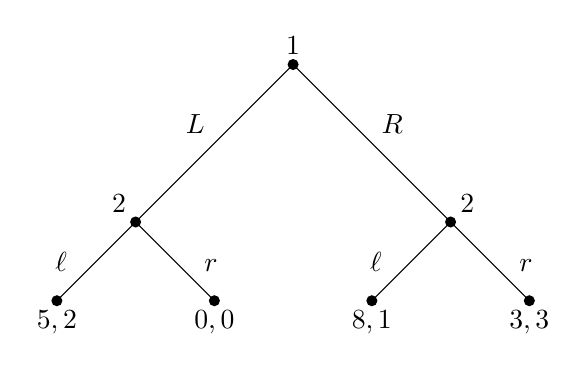
\begin{tikzpicture}
    \fill (0,0) circle (2pt) node [above] {$1$};
    \fill (-2,-2) circle (2pt) node [above left] {$2$};
    \fill (2,-2) circle (2pt) node [above right] {$2$};
    \fill (-3,-3) circle (2pt) node [below] {$5,2$};
    \fill (-1,-3) circle (2pt) node [below] {$0,0$};
    \fill (1,-3) circle (2pt) node [below] {$8,1$};
    \fill (3,-3) circle (2pt) node [below] {$3,3$};

    \draw (0,0) -- (-2,-2) node [midway,above left] {$L$};
    \draw (-2,-2) -- (-3,-3) node [near end,above left] {$\ell$};
    \draw (-2,-2) -- (-1,-3) node [near end,above right] {$r$};
    \draw (0,0) -- (2,-2) node [midway,above right] {$R$};
    \draw (2,-2) -- (1,-3) node [near end,above left] {$\ell$};
    \draw (2,-2) -- (3,-3) node [near end,above right] {$r$};
  \end{tikzpicture}
\end{center}

\begin{enumerate}
  \item Beschreiben Sie in Worten die Spielabfolge, potentielle Aktionen der Agenten und
    deren Informationen auf jeder Stufe.

  \item Erklären Sie den Unterschied zwischen einer Aktion und einer Strategie. Geben Sie
    für jeden Spieler ein Beispiel einer Aktion und ein Beispiel einer Strategie.

  \item Definieren Sie das Lösungskonzept Nash-GG (NGG). Was sind die reinen NGG dieses
    Spiels? Was sind die Ergebnisse dieser NGG?

  \item Definieren Sie ein Teilspiel und ein teilspielperfektes Nash-GG (SPNE) informell.
    Was sind die reinen SPNE dieses Spiels? Was sind die Ergebnisse dieser SPNE?

  \item Finden Sie das Konzept eines SPNE attraktiv? Ist es im Kontext dieses Spiels
    angemessen?
\end{enumerate}

\subparagraph{Lösung}%

\begin{enumerate}
  \item Anfangs ist Spieler 1 am Zug und entscheidet zwischen den möglichen Aktionen $L$
    und $R$.
    Danach ist Spieler 2 am Zug und weiß, ob Spieler 1 $L$ oder $R$ gespielt hat.
    Spieler 2 entscheidet, ob er $\ell$ oder $r$ spielt.

  \item Eine Aktion wird nur an einem Knoten im Spielbaum ausgeführt, während eine
    Strategie ein „Plan für alle Eventualitäten ist.“

    Spieler 1 hat z.\,B. die Aktion $L$ und auch die Strategie $L$.
    Spieler 2 hat z.\,B. die Aktion $\ell$ nachdem Spieler 1 $L$ gespielt hat
    und die Strategie $rr$.

  \item Ein Nash-Gleichgewicht ist eine Kombination von Strategien, wobei jeder Spieler
    genau eine Strategie wählt, von der aus es für keinen Spieler sinnvoll ist, von der
    gewählten Strategie als einziger abzuweichen.

    Zur Bestimmung der Nash-Gleichgewichte wird das extensive Spiel in ein statisches
    Spiel überführt:

    \begin{center}
      \begin{tabular}{cccccc}
        & & \multicolumn{4}{c}{Spieler 2}\\
        & & $\ell \ell$ & $\ell r$ & $r \ell$ & $rr$\\
        \cmidrule{3-6}
        \multirow{2}{*}{Spieler 1}
        & $L$ & $5,\underline{2}$ & $\underline{5},\underline{2}$ & $0,0$ & $0,0$\\
        \cmidrule{3-6}
        & $R$ & $\underline{8},1$ & $3,\underline{3}$ & $\underline{8},1$ &
        $\underline{3},\underline{3}$\\
        \cmidrule{3-6}
      \end{tabular}
    \end{center}

    Es gilt $\text{NGG} = \{(L, \ell r), (R, rr)\}$.

    Angenommen Spieler 2 entscheidet sich $rr$ zu spielen und kündigt dies offen für
    Spieler 1 an.
    Falls Spieler 1 $R$ spielt, erhält Spieler 2 die größtmögliche Auszahlung.
    Falls Spieler 1 jedoch $L$ spielt, dann erhält Spieler 2 die kleinstmögliche
    Auszahlung, obwohl Spieler 2 im linken Teilspiel durch die Aktion $\ell$ eine größere
    Auszahlung erhalten könnte.
    Die Ankündigung von Spieler 2 $rr$ zu spielen dient als \emph{Drohung} um Spieler 1 zu
    $R$ zu zwingen.
    Diese Drohung ist jedoch unglaubwürdig, weil es für Spieler 2 im linken Teilspiel
    rational wäre $\ell$ zu spielen.

  \item Ein Teilspiel ist ein Spiel, das in einem einzelnen Entscheidungsknoten des
    Spielbaums beginnt und alle Knoten enthält, die diesem Knoten nachfolgen, wobei keine
    Informationsbezirke getrennt werden dürfen.
    Ein Nash-Gleichgewicht ist \emph{teilspielperfekt}, wenn es ein Nash-Gleichgewicht in
    jedem Teilspiel induziert.

    In diesem Spiel gilt $\text{SPNE} = \{(L, \ell r)\}$.

  \item Ja und ja.
\end{enumerate}

\paragraph{Aufgabe 3}%
\label{par:aufgabe_3}

Betrachten Sie folgendes Spiel in extensiver Form:
\begin{center}
  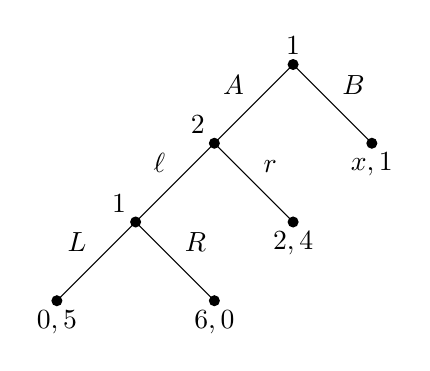
\begin{tikzpicture}
    \fill (0,0) circle (2pt) node [below] {$0,5$};
    \fill (2,0) circle (2pt) node [below] {$6,0$};
    \fill (1,1) circle (2pt) node [above left] {$1$};
    \fill (3,1) circle (2pt) node [below] {$2,4$};
    \fill (2,2) circle (2pt) node [above left] {$2$};
    \fill (4,2) circle (2pt) node [below] {$x,1$};
    \fill (3,3) circle (2pt) node [above] {$1$};

    \draw (3,3) -- (2,2) node [midway, above left] {$A$};
    \draw (3,3) -- (4,2) node [midway, above right] {$B$};
    \draw (2,2) -- (1,1) node [midway, above left] {$\ell$};
    \draw (2,2) -- (3,1) node [midway, above right] {$r$};
    \draw (1,1) -- (0,0) node [midway, above left] {$L$};
    \draw (1,1) -- (2,0) node [midway, above right] {$R$};
  \end{tikzpicture}
\end{center}

\begin{enumerate}
  \item Bestimmen Sie die Strategien der Spieler.
  \item Finden Sie die Menge der NGG dieses Spiels.
  \item Finden Sie die Menge der SPNE dieses Spiels für $x = 7,4,1$.
  \item Finden Sie das Konzept eines SPNE attraktiv?
    Vergleichen Sie die Situation für $x=7,4,1$.
\end{enumerate}

\subparagraph{Lösung}%

\begin{enumerate}
  \item Spieler 1 hat folgende Strategien: $AL, AR, BL, BR$.
    Spieler 2: $\ell, r$.

  \item Wir betrachten die Nash-Gleichgewichte für $x=7,4,1$ (auch wenn die
    Aufgabenstellung diese Werte für $x$ nicht vorgegeben hat):
    \begin{center}
      \begin{minipage}{0.30\textwidth}
        \begin{tabular}{cccc}
          & & \multicolumn{2}{c}{2}\\
          & $x=7$ & $\ell$ & $r$\\
          \multirow{4}{*}{1}
          & $AL$ & $0,\underline{5}$ & $2,4$\\
          & $AR$ & $6,0$ & $2,\underline{4}$\\
          & $BL$ & $\underline{x},\underline{1}$ & $\underline{x},\underline{1}$\\
          & $BR$ & $\underline{x},\underline{1}$ & $\underline{x},\underline{1}$
        \end{tabular}
      \end{minipage}
      \begin{minipage}{0.30\textwidth}
        \begin{tabular}{cccc}
          & & \multicolumn{2}{c}{2}\\
          & $x=4$ & $\ell$ & $r$\\
          \multirow{4}{*}{1}
          & $AL$ & $0,\underline{5}$ & $2,4$\\
          & $AR$ & $\underline{6},0$ & $2,\underline{4}$\\
          & $BL$ & $x,\underline{1}$ & $\underline{x},\underline{1}$\\
          & $BR$ & $x,\underline{1}$ & $\underline{x},\underline{1}$
        \end{tabular}
      \end{minipage}
      \begin{minipage}{0.30\textwidth}
        \begin{tabular}{cccc}
          & & \multicolumn{2}{c}{2}\\
          & $x=1$ & $\ell$ & $r$\\
          \multirow{4}{*}{1}
          & $AL$ & $0,\underline{5}$ & $\underline{2},4$\\
          & $AR$ & $\underline{6},0$ & $\underline{2},\underline{4}$\\
          & $BL$ & $x,\underline{1}$ & $x,\underline{1}$\\
          & $BR$ & $x,\underline{1}$ & $x,\underline{1}$
        \end{tabular}
      \end{minipage}
    \end{center}
    \begin{align*}
      \underset{x=7}{\text{NGG}} & = \{(BL, \ell), (BL, r), (BR, \ell), (BR, r)\}\\
      \underset{x=4}{\text{NGG}} & = \{(BL, r), (BR, r)\}\\
      \underset{x=1}{\text{NGG}} & = \{(AR, r)\}
    \end{align*}

  \item Per Rückwärtsinduktion ergeben sich folgende SPNE:
    \begin{align*}
      \underset{x \in \{4,7\}}{\text{SPNE}} & = \{(BR, r)\}\\
      \underset{x=1}{\text{SPNE}} & = \{(AR, r)\}
    \end{align*}
\end{enumerate}


\paragraph{Aufgabe 4}%
\label{par:aufgabe_4}

Betrachten Sie folgendes Spiel in extensiver Form:
\begin{center}
  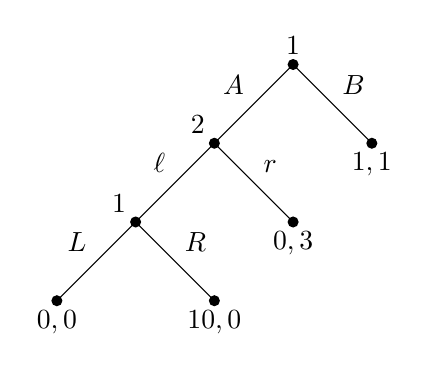
\begin{tikzpicture}
    \fill (0,0) circle (2pt) node [below] {$0,0$};
    \fill (2,0) circle (2pt) node [below] {$10,0$};
    \fill (1,1) circle (2pt) node [above left] {$1$};
    \fill (3,1) circle (2pt) node [below] {$0,3$};
    \fill (2,2) circle (2pt) node [above left] {$2$};
    \fill (4,2) circle (2pt) node [below] {$1,1$};
    \fill (3,3) circle (2pt) node [above] {$1$};

    \draw (3,3) -- (2,2) node [midway, above left] {$A$};
    \draw (3,3) -- (4,2) node [midway, above right] {$B$};
    \draw (2,2) -- (1,1) node [midway, above left] {$\ell$};
    \draw (2,2) -- (3,1) node [midway, above right] {$r$};
    \draw (1,1) -- (0,0) node [midway, above left] {$L$};
    \draw (1,1) -- (2,0) node [midway, above right] {$R$};
  \end{tikzpicture}
\end{center}

\begin{enumerate}
  \item Finden Sie die Menge NGG dieses Spiels.
  \item Finden Sie die Menge der SPNE dieses Spiels.
  \item Nehmen Sie nun an, dass Spieler 2 mit Wahrscheinlichkeit $\beta \in (0,1)$
    irrational ist und mit der selben Wahrscheinlichkeit $\ell, r$ wählt.
    Wie groß muss $\beta$ sein, damit es für Spieler $1$ optimal ist $A$ zu wählen?
\end{enumerate}

\subparagraph{Lösung}%

\begin{enumerate}
  \item Zur Bestimmung der NGG:
    \begin{center}
      \begin{tabular}{cccc}
        & & \multicolumn{2}{c}{2}\\
        & & $\ell$ & $r$\\
        \multirow{4}{*}{1}
        & $AL$ & $0,0$ & $0,\underline{3}$\\
        & $AR$ & $\underline{10},0$ & $0,\underline{3}$\\
        & $BL$ & $1,\underline{1}$ & $\underline{1},\underline{1}$\\
        & $BR$ & $1,\underline{1}$ & $\underline{1},\underline{1}$
      \end{tabular}
    \end{center}
    Damit gilt $\text{NGG} = \{(BL, r), (BR,r)\}$.

  \item Per Rückwärtsinduktion ergibt sich: $\text{SPNE} = \{(BR,r)\}$.

  \item Beim folgenden Teilspiel wählt Spieler 1 immer $R$, da Spieler 1 rational ist:
    \begin{center}
      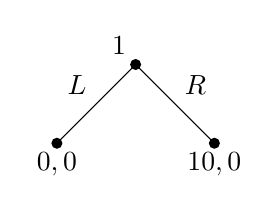
\begin{tikzpicture}
        \fill (0,0) circle (2pt) node [below] {$0,0$};
        \fill (2,0) circle (2pt) node [below] {$10,0$};
        \fill (1,1) circle (2pt) node [above left] {$1$};

        \draw (1,1) -- (0,0) node [midway, above left] {$L$};
        \draw (1,1) -- (2,0) node [midway, above right] {$R$};
      \end{tikzpicture}
    \end{center}
    Beim sich daraus ergebenden Teilspiel
    \begin{center}
      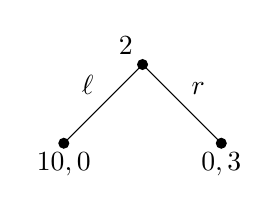
\begin{tikzpicture}
        \fill (1,1) circle (2pt) node [below] {$10,0$};
        \fill (3,1) circle (2pt) node [below] {$0,3$};
        \fill (2,2) circle (2pt) node [above left] {$2$};

        \draw (2,2) -- (1,1) node [midway, above left] {$\ell$};
        \draw (2,2) -- (3,1) node [midway, above right] {$r$};
      \end{tikzpicture}
    \end{center}
    ist Spieler 2 mit der Wahrscheinlichkeit $\beta$ irrational und wählt mit der
    Wahrscheinlichkeit $\frac{1}{2}$ entweder $\ell$ oder $r$.
    Daraus ergeben sich folgende Erwartungsnutzen:
    \begin{align*}
      EU_2 & = \beta(\frac{1}{2} \cdot 0 + \frac{1}{2} \cdot 3) + (1-\beta) \cdot 3
             = 3 - \frac{3}{2}\beta\\
      EU_1 & = \beta(\frac{1}{2} \cdot 10 + \frac{1}{2} \cdot 0) + (1-\beta) \cdot 0
             = 5 \beta
    \end{align*}
    Beim sich daraus ergebenden Teilspiel auf oberster Ebene
    \begin{center}
      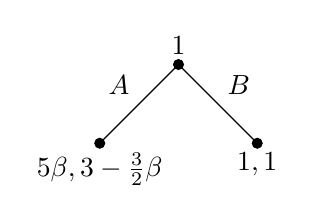
\begin{tikzpicture}
        \fill (2,2) circle (2pt) node [below] {$5\beta, 3-\frac{3}{2}\beta$};
        \fill (4,2) circle (2pt) node [below] {$1,1$};
        \fill (3,3) circle (2pt) node [above] {$1$};

        \draw (3,3) -- (2,2) node [midway, above left] {$A$};
        \draw (3,3) -- (4,2) node [midway, above right] {$B$};
      \end{tikzpicture}
    \end{center}
    fragt sich Spieler 1: für welches $\beta$ gilt $5\beta > 1$?
    Für $\beta > \frac{1}{5}$.
\end{enumerate}

\paragraph{Aufgabe 5}%
\label{par:aufgabe_5}

In einer Amerikanischen Fernsehshow wird den Spielern die Wahl zwischen dem Öffnen einer
von drei Türen (rot, grün, blau) angeboten.
Hinter einer Tür verbirgt sich ein Preis, hinter den anderen nichts.
Die Spieler haben keinen Grund anzunehmen, dass eine der Türen mit höherer
Wahrscheinlichkeit zu einem Preis führt als eine andere.
Der Quizmaster weiß, hinter welcher Tür der Preis liegt.
Nachdem ein Spieler eine der Türen gewählt (aber noch nicht geöffnet) hat, \emph{muss} der
Quizmaster eine der anderen Türen öffnen.
Der Spieler kann sich dann entscheiden, ob er bei der von ihm ursprünglich gewählten Tür
bleibt, oder ob er zu einer anderen Tür wechselt.
Nehmen Sie an, dass die Spieler die Wahrscheinlichkeit den Preis zu bekommen maximieren,
während der Quizmaster diese Wahrscheinlichkeit minimieren möchte.

\begin{enumerate}
  \item Beschreiben Sie eine optimale Strategie des Quizmasters.
    Nehmen Sie im Weiteren an, dass der Quizmaster diese Strategie verfolgt.

  \item Was sollte der Spieler tun, wenn er gefragt wird, ob er wechseln möchte?
    Begründen Sie Ihre Antwort.
\end{enumerate}

\subsection{Serie 7}%
\label{sub:serie_7}

\paragraph{Aufgabe 1}%
\label{par:serie_7_aufgabe_1}

Zwei Personen (1 und 2) wählen aus drei Alternativen ($A, B, C$) eine mit Hilfe des
folgenden Verfahrens aus: zuerst streicht Person 1 eine Alternative.
Dann streicht Person 2 eine der verbliebenen Alternativen.
Die dann noch verbliebene Alternative gilt als ausgewählt.
Person 1 zieht die Alternative $A$ der Alternative $B$ vor, die sie wiederum der
Alternative $C$ vorzieht.
Person 2 ordnet die Alternativen gerade umgekehrt.

\begin{enumerate}
  \item Stellen Sie diese Situation durch einen Spielbaum dar.
  \item Bestimmen Sie durch Rückwärtsinduktion das teilspielperfekte Gleichgewicht.
  \item Gibt es andere Nash-Gleichgewichte?
    Gibt es welche, in denen eine andere Alternative als in dem teilspielperfekten
    Gleichgewicht ausgewählt wird?
\end{enumerate}

\subparagraph{Lösung}%

\begin{enumerate}
  \item Es entsteht folgender Spielbaum:
    \begin{center}
      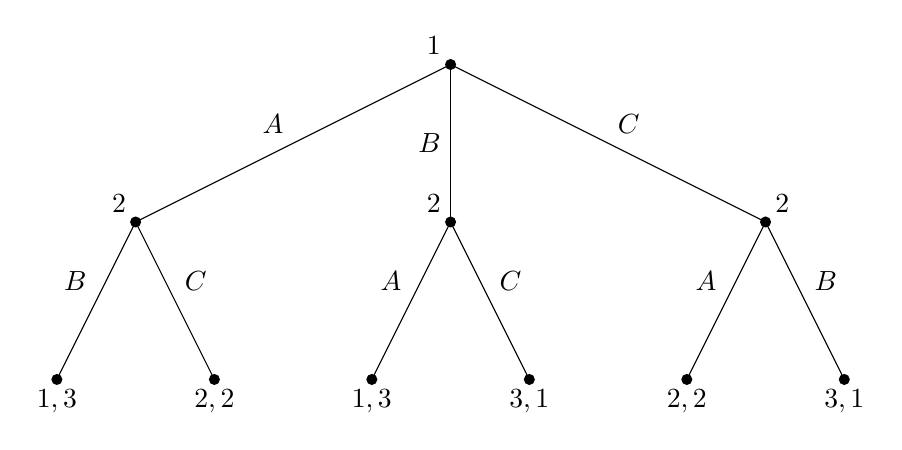
\begin{tikzpicture}
        \fill (0,0) circle (2pt) node [below] {$1,3$};
        \fill (2,0) circle (2pt) node [below] {$2,2$};
        \fill (4,0) circle (2pt) node [below] {$1,3$};
        \fill (6,0) circle (2pt) node [below] {$3,1$};
        \fill (8,0) circle (2pt) node [below] {$2,2$};
        \fill (10,0) circle (2pt) node [below] {$3,1$};

        \fill (1,2) circle (2pt) node [above left] {2};
        \fill (5,2) circle (2pt) node [above left] {2};
        \fill (9,2) circle (2pt) node [above right] {2};

        \fill (5,4) circle (2pt) node [above left] {1};

        \draw (5,4) -- (1,2) node [midway, above left] {$A$};
        \draw (5,4) -- (5,2) node [midway, left] {$B$};
        \draw (5,4) -- (9,2) node [midway, above right] {$C$};

        \draw (1,2) -- (0,0) node [midway, above left] {$B$};
        \draw (1,2) -- (2,0) node [midway, above right] {$C$};
        \draw (5,2) -- (4,0) node [midway, above left] {$A$};
        \draw (5,2) -- (6,0) node [midway, above right] {$C$};
        \draw (9,2) -- (8,0) node [midway, above left] {$A$};
        \draw (9,2) -- (10,0) node [midway, above right] {$B$};
      \end{tikzpicture}
    \end{center}

  \item Es ergeben sich folgende teilspielperfekte Gleichgewichte:
    \begin{center}
      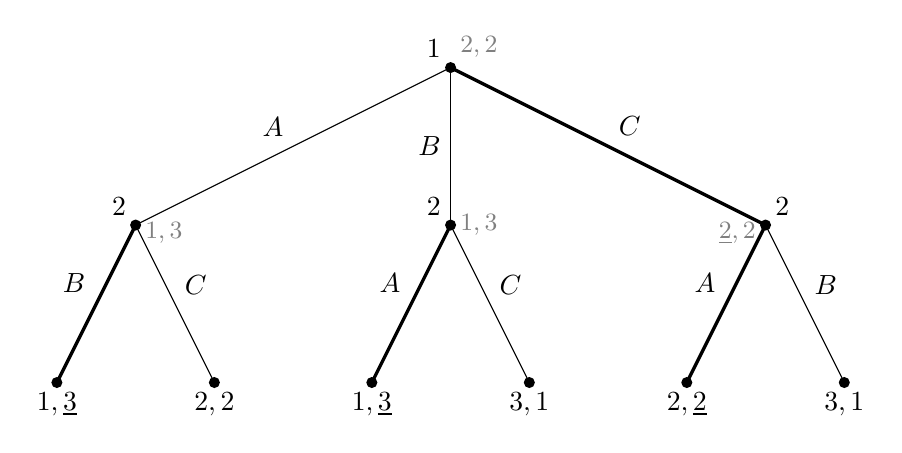
\begin{tikzpicture}
        \fill (0,0) circle (2pt) node [below] {$1,\underline{3}$};
        \fill (2,0) circle (2pt) node [below] {$2,2$};
        \fill (4,0) circle (2pt) node [below] {$1,\underline{3}$};
        \fill (6,0) circle (2pt) node [below] {$3,1$};
        \fill (8,0) circle (2pt) node [below] {$2,\underline{2}$};
        \fill (10,0) circle (2pt) node [below] {$3,1$};

        \fill (1,2) circle (2pt)
          node [above left] {2}
          node [right, yshift=-3pt, gray] {\small $1, 3$};
        \fill (5,2) circle (2pt)
          node [above left] {2}
          node [right, gray] {\small $1, 3$};
        \fill (9,2) circle (2pt)
          node [above right] {2}
          node [left, yshift=-3pt, gray] {\small $\underline{2}, 2$};

        \fill (5,4) circle (2pt)
          node [above left] {1}
          node [above right, gray] {\small $2, 2$};

        \draw (5,4) -- (1,2) node [midway, above left] {$A$};
        \draw (5,4) -- (5,2) node [midway, left] {$B$};
        \draw [very thick] (5,4) -- (9,2) node [midway, above right] {$C$};

        \draw [very thick] (1,2) -- (0,0) node [midway, above left] {$B$};
        \draw (1,2) -- (2,0) node [midway, above right] {$C$};
        \draw [very thick] (5,2) -- (4,0) node [midway, above left] {$A$};
        \draw (5,2) -- (6,0) node [midway, above right] {$C$};
        \draw [very thick] (9,2) -- (8,0) node [midway, above left] {$A$};
        \draw (9,2) -- (10,0) node [midway, above right] {$B$};
      \end{tikzpicture}
    \end{center}
    Damit gilt $\text{SPNE} = \{(C, BAA)\}$.

  \item Wir betrachten alle möglichen Strategien der Spieler:
    \begin{center}
      \begin{tabular}{cccccccccc}
        & & \multicolumn{8}{c}{Spieler 2}\\
        & & $BAA$ & $BAB$ & $BCA$ & $BCB$ & $CAA$ & $CAB$ & $CCA$ & $CCB$\\
        \cmidrule{3-10}
        \multirow{3}{*}{Spieler 1}
        & $A$ & $1,\underline{3}$ & $1,\underline{3}$
              & $1,\underline{3}$ & $1,\underline{3}$
              & $\underline{2},2$ & $2,2$
              & $2,2$ & $2,2$\\
        \cmidrule{3-10}
        & $B$ & $1,\underline{3}$ & $1,\underline{3}$
              & $\underline{3},1$ & $\underline{3},1$
              & $1,\underline{3}$ & $1,\underline{3}$
              & $\underline{3},1$ & $\underline{3},1$\\
        \cmidrule{3-10}
        & $C$ & \framebox{$\underline{2},\underline{2}$} & $\underline{3},1$
              & $2,\underline{2}$ & $\underline{3},1$
              & \framebox{$\underline{2},\underline{2}$} & $\underline{3},1$
              & $2,\underline{2}$ & $\underline{3},1$\\
        \cmidrule{3-10}
      \end{tabular}
    \end{center}
    Damit ist $(C,CAA)$ ein anderes Nash-Gleichgewicht mit reinen Strategien.

    Spieler 2 könnte auch eine gemischte Strategie der beiden Gleichgewichte spielen,
    da Spieler 2 mit jeder Wahrscheinlichkeit $p \in (0,1]$
    für die gemischte Strategie $(C, \langle p \cdot BAA, (1-p) \cdot CAA\rangle)$
    die Auszahlung
    \begin{align*}
      p \cdot 3 + (1-p) \cdot 2 = 2+p
    \end{align*}
    erhält und diese immer echt größer als die Auszahlung der reinen Strategien ist.
\end{enumerate}

\paragraph{Aufgabe 2}%
\label{par:serie_7_aufgabe_2}

Spieler 1 und 2 nehmen an einer Versteigerung teil.
Der Gewinner der Versteigerung erhält $x > 0$ Euro.
Die Regeln sind wie folgt: die Spieler bieten abwechselnd (beginnend mit Spieler 1) bis
entweder ein Spieler passt oder der Betrag von $x-1$ Euro geboten wurde.
Ist ein Spieler am Zug kann er entweder das letzte Gebot um einen Euro überbieten (bei
Beginn des Spiels gilt 0 als das letzte Gebot) oder passen.
\emph{Jeder} Spieler muss \emph{jedes} Gebot, das er macht, umgehend bezahlen
(hat Spieler 1 z.\,B. in einer Partie 1 und 3 (und sonst nichts) geboten, so muss er 4
Euro bezahlen).
Passt Spieler 1 im ersten Zug, so ist Spieler 2 der Gewinner.
Ansonsten ist derjenige Spieler der Gewinner, der das höchste Gebot abgibt.
Die Auszahlung des Gewinners ist $x$ abzüglich der Summe seiner Gebote.
Die Auszahlung des Verlierers ist $0$ abzüglich der Summe seiner Gebote.

\begin{enumerate}
  \item Bestimmen Sie für $x=4$ die teilspielperfekten Gleichgewichte dieses Spiels.
  \item Wiederholen Sie die Aufgabe für $x=5$.
\end{enumerate}

\subparagraph{Lösung}%

\begin{enumerate}
  \item Bei $x=4$ ergibt sich folgender Spielbaum:
    \begin{center}
      \begin{tikzpicture}
        \fill (0,0) circle (2pt) node [above left] {1};

        \fill (-1,-2) circle (2pt) node [above left] {2};
        \fill (1,-2) circle (2pt) node [below] {$0,4$};

        \draw (0,0) -- (-1,-2) node [midway, above left] {$b$};
        \draw (0,0) -- (1,-2) node [midway, above right] {$p$};

        \fill (-2,-4) circle (2pt) node [above left] {1};
        \fill (0,-4) circle (2pt) node [below] {$3,0$};

        \draw (-1,-2) -- (-2,-4) node [midway, above left] {$b$};
        \draw (-1,-2) -- (0,-4) node [midway, above right] {$p$};

        \fill (-3,-6) circle (2pt) node [below] {$0,-2$};
        \fill (-1,-6) circle (2pt) node [below] {$-1,-2$};

        \draw (-2,-4) -- (-3,-6) node [midway, above left] {$b$};
        \draw (-2,-4) -- (-1,-6) node [midway, above right] {$p$};
      \end{tikzpicture}
    \end{center}
    Und folgende teilspielperfekte Gleichgewichte:
    \begin{center}
      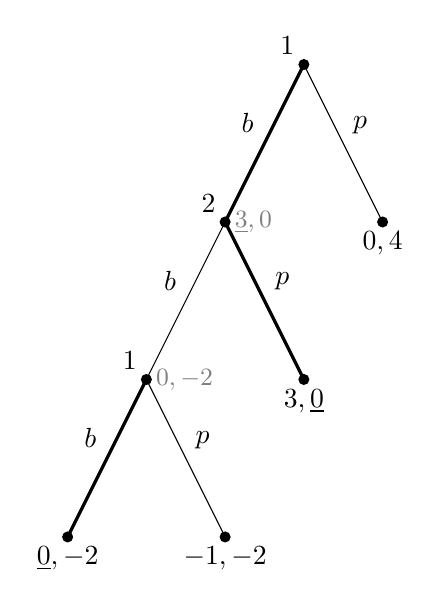
\begin{tikzpicture}
        \fill (0,0) circle (2pt) node [above left] {1};

        \fill (-1,-2) circle (2pt)
          node [above left] {2}
          node [right, gray] {\small $\underline{3},0$};
        \fill (1,-2) circle (2pt) node [below] {$0,4$};

        \draw [very thick] (0,0) -- (-1,-2) node [midway, above left] {$b$};
        \draw (0,0) -- (1,-2) node [midway, above right] {$p$};

        \fill (-2,-4) circle (2pt)
          node [above left] {1}
          node [right, gray] {\small $0,-2$};
        \fill (0,-4) circle (2pt) node [below] {$3,\underline{0}$};

        \draw (-1,-2) -- (-2,-4) node [midway, above left] {$b$};
        \draw [very thick] (-1,-2) -- (0,-4) node [midway, above right] {$p$};

        \fill (-3,-6) circle (2pt) node [below] {$\underline{0},-2$};
        \fill (-1,-6) circle (2pt) node [below] {$-1,-2$};

        \draw [very thick] (-2,-4) -- (-3,-6) node [midway, above left] {$b$};
        \draw (-2,-4) -- (-1,-6) node [midway, above right] {$p$};
      \end{tikzpicture}
    \end{center}
    Es gilt $\text{SPNE} = \{(bb,p)\}$.

  \item $x=5$:
    \begin{center}
      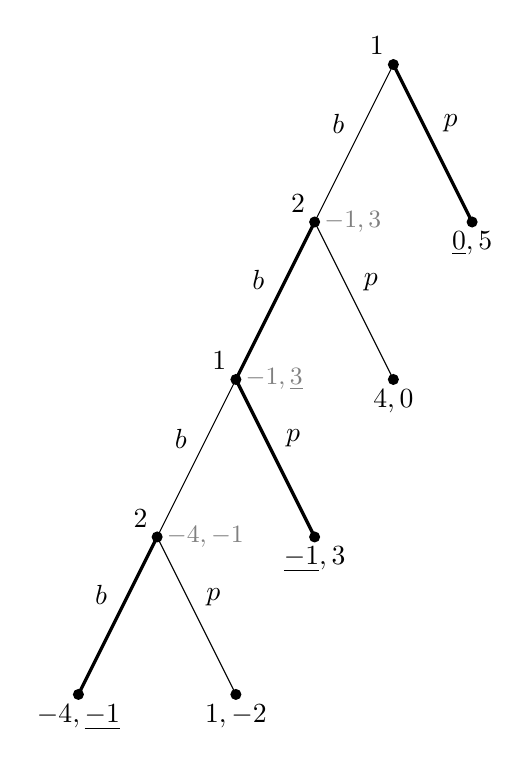
\begin{tikzpicture}
        \fill (0,0) circle (2pt) node [above left] {1};

        \fill (-1,-2) circle (2pt)
          node [above left] {2}
          node [right, gray] {\small $-1,3$};
        \fill (1,-2) circle (2pt) node [below] {$\underline{0},5$};

        \draw (0,0) -- (-1,-2) node [midway, above left] {$b$};
        \draw [very thick] (0,0) -- (1,-2) node [midway, above right] {$p$};

        \fill (-2,-4) circle (2pt)
          node [above left] {1}
          node [right, gray] {\small $-1,\underline{3}$};
        \fill (0,-4) circle (2pt) node [below] {$4,0$};

        \draw [very thick] (-1,-2) -- (-2,-4) node [midway, above left] {$b$};
        \draw (-1,-2) -- (0,-4) node [midway, above right] {$p$};

        \fill (-3,-6) circle (2pt)
          node [above left] {2}
          node [right, gray] {\small $-4,-1$};
        \fill (-1,-6) circle (2pt) node [below] {$\underline{-1},3$};

        \draw (-2,-4) -- (-3,-6) node [midway, above left] {$b$};
        \draw [very thick] (-2,-4) -- (-1,-6) node [midway, above right] {$p$};

        \fill (-4,-8) circle (2pt) node [below] {$-4,\underline{-1}$};
        \fill (-2,-8) circle (2pt) node [below] {$1,-2$};

        \draw [very thick] (-3,-6) -- (-4,-8) node [midway, above left] {$b$};
        \draw (-3,-6) -- (-2,-8) node [midway, above right] {$p$};
      \end{tikzpicture}
    \end{center}
    Daraus folgt $\text{SPNE} = \{(pp,bb)\}$.
\end{enumerate}

\paragraph{Aufgabe 3}%
\label{par:serie_7_aufgabe_3}

Nehmen Sie an, dass in einer Variante des Spiels \emph{Bach oder Strawinski}
\begin{center}
  \begin{tabular}{cccc}
    & & \multicolumn{2}{c}{Spieler 2}\\
    & & $B$ & $S$\\
    \cmidrule{3-4}
    \multirow{2}{*}{Spieler 1}
    & $B$ & $2,1$ & $0,0$\\
    \cmidrule{3-4}
    & $S$ & $0,0$ & $1,2$\\
    \cmidrule{3-4}
  \end{tabular}
\end{center}
die Spieler ihre Aktionen nicht gleichzeitig sondern hintereinander wählen (Spieler 1 ist
zuerst am Zug, Spieler 2 kann die Aktion von Spieler 1 beobachten, bevor er seine Aktion
wählt).
\begin{enumerate}
  \item Bestimmen Sie die strategische Form dieses Spiels.
  \item Bestimmen Sie die Nash-Gleichgewichte in reinen Strategien.
  \item Welches dieser NGG ist teilspielperfekt?
\end{enumerate}

\subparagraph{Lösung}%
\begin{enumerate}
  \item Das Spiel hat folgende strategische Form:
    \begin{center}
      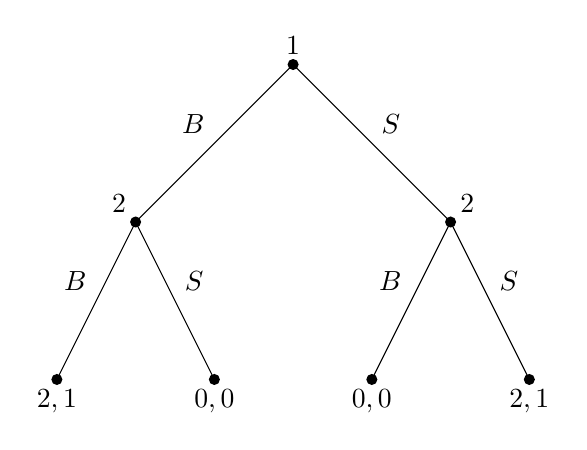
\begin{tikzpicture}
        \fill (0,0) circle (2pt) node [above] {1};

        \fill (-2,-2) circle (2pt) node [above left] {2};
        \fill (2,-2) circle (2pt) node [above right] {2};

        \draw (0,0) -- (-2,-2) node [midway, above left] {$B$};
        \draw (0,0) -- (2,-2) node [midway, above right] {$S$};

        \fill (-3,-4) circle (2pt) node [below] {$2,1$};
        \fill (-1,-4) circle (2pt) node [below] {$0,0$};
        \fill (1,-4) circle (2pt) node [below] {$0,0$};
        \fill (3,-4) circle (2pt) node [below] {$2,1$};

        \draw (-2,-2) -- (-3,-4) node [midway, above left] {$B$};
        \draw (-2,-2) -- (-1,-4) node [midway, above right] {$S$};
        \draw (2,-2) -- (1,-4) node [midway, above left] {$B$};
        \draw (2,-2) -- (3,-4) node [midway, above right] {$S$};
      \end{tikzpicture}
    \end{center}

  \item Zur Bestimmung der Nash-Gleichgewichte betrachten wir alle möglichen Strategien
    der Spieler:
    \begin{center}
      \begin{tabular}{cccccc}
        & & \multicolumn{4}{c}{Spieler 2}\\
        & & $BB$ & $BS$ & $SB$ & $SS$\\
        \cmidrule{3-6}
        \multirow{2}{*}{Spieler 1}
        & $B$ & $\underline{2},\underline{1}$ & $\underline{2},\underline{1}$
              & $0,0$ & $0,0$\\
        \cmidrule{3-6}
        & $S$ & $0,0$ & $1,\underline{2}$ & $0,0$ & $\underline{1},\underline{2}$\\
        \cmidrule{3-6}
      \end{tabular}
    \end{center}
    Damit gilt $\text{NGG} = \{(B,BB), (B,BS), (S, SS)\}$.

  \item Von diesen Gleichgewichten ist nur $(B, BS)$ teilspielperfekt.
\end{enumerate}

\subsection{Serie 8}%
\label{sub:serie_8}

\paragraph{Aufgabe 1}%
\label{par:serie_8_aufgabe_1}

Spieler 1 und 2 wechseln sich in einem Spiel mit vollkommener Information darin ab
(beginnend mit Spieler 1), Steine von einem Haufen wegzunehmen.
Zu Beginn des Spiels sind $n > 0$ Steine auf dem Haufen.
Ein Spieler, der am Zug ist, kann einen oder zwei Steine wegnehmen.
Das Spiel endet, wenn kein Stein mehr auf dem Haufen liegt.
Der Spieler, der den letzten Stein wegnimmt, ist der Gewinner.
Die Auszahlung des Gewinners ist 1; die des Verlierers ist 0.
Für $n = 1$ und $n = 2$ gewinnt (in einem teilspielperfekten Gleichgewicht) offenkundig
Spieler 1 dieses Spiel.

\begin{enumerate}
  \item Wer gewinnt für $n = 3$? Wer für $n = 4$?
  \item Können Sie den Gewinner für beliebiges $n$ bestimmen?
\end{enumerate}

\subparagraph{Lösung}%

\begin{enumerate}
  \item Für $n=3$:
    \begin{center}
      \begin{tikzpicture}[
          level/.style={sibling distance=60mm/#1},
        ]
        \node {$1_{\color{mygray}{3}}$}
          child {
            node {$2_{\color{mygray}{2}}$}
            child {
              node {$1_{\color{mygray}{1}}$}
              child {
                node {$1,0$}
              }
              edge from parent node [above left] {1}
            }
            child [very thick] {
              node {$0, 1$}
              edge from parent node [above right] {2}
            }
            edge from parent node [above left] {1}
          }
          child {
            node {$2_{\color{mygray}{1}}$}
            child [very thick] {
              node {$0,1$}
              edge from parent node [right] {1}
            }
            edge from parent node [above right] {2}
          }
        ;
      \end{tikzpicture}
    \end{center}
    Bei $n=3$ gewinnt immer Spieler 2.

    Für $n=4$:
    \begin{center}
      \begin{tikzpicture}[
          level/.style={sibling distance=60mm/#1},
        ]
        \node {$1_{\color{mygray}{4}}$}
          child {
            node {$2_{\color{mygray}{3}}$}
            child {
              node {$1_{\color{mygray}{2}}$}
              child [very thick] {
                node {$1,0$}
              }
              edge from parent node [above left] {1}
            }
            child {
              node {$1_{\color{mygray}{1}}$}
              child {
                node {$1,0$}
                edge from parent node [right] {1}
              }
              edge from parent node [above right] {2}
            }
            edge from parent node [above left] {1}
          }
          child {
            node {$2_{\color{mygray}{2}}$}
            child [very thick] {
              node {$0,1$}
            }
            edge from parent node [above right] {2}
          }
        ;
      \end{tikzpicture}
    \end{center}
    Bei $n=4$ gewinnt immer Spieler 1 mit der Strategie 11 bzw. 12.

\end{enumerate}


\paragraph{Aufgabe 2}%
\label{par:serie_8_aufgabe_2}

In einem Spiel mit vollkommener Information gibt es drei Felder: $A, B$ und $C$.
Spieler 1 beginnt das Spiel, indem er auf die Felder positive Geldbeträge
$(x_A, x_B, x_C)$ legt.
Danach ist Spieler 2 am Zug und kann positive Geldbeträge $(y_A, y_B, y_C)$ auf die Felder
legen.
Damit endet das Spiel.
Der Gewinner ist der Spieler, der die meisten Felder gewinnt.
Spieler 1 gewinnt das Feld $f \in \{A,B,C\}$, wenn $x_f > y_f$ gilt;
ansonsten gewinnt Spieler 2 das Feld.
Gewinnt Spieler $i$, erhält er einen Preis in Höhe von $V_i > 0$.
Jeder Spieler muss die Summe seiner Gebote bezahlen.
Wenn Spieler 1 gewinnt, ist seine Auszahlung also
\begin{align*}
  V_1 - x_A - x_B - x_C,
\end{align*}
wenn er verliert, ist sie
\begin{align*}
  - x_A - x_B - x_C,
\end{align*}
Die Auszahlungen von Spieler 2 sind entsprechend.

\begin{enumerate}
  \item Bestimmen Sie das (jeweils eindeutig bestimmte) Ergebnis der teilspielperfekten
    Gleichgewichte für den Fall $V_1 = V_2 = 300$.
    (Hinweis: eine vollständige Bestimmung der Gleichgewichtsstrategien ist hierfür nicht
    erforderlich; Sie dürfen in der Bearbeitung unterstellen, dass es teilspielperfekte
    Gleichgewichte gibt.)
  \item Wiederholen Sie die Aufgabe für den Fall $V_1 = 300, V_2 = 100$.
\end{enumerate}

\paragraph{Aufgabe 3}%
\label{par:serie_8_aufgabe_3}

Betrachten Sie das folgende Verhandlungsspiel.
In Runde 1 macht Spieler 1 ein Angebot $x \in [0, 1]$; daraufhin entscheidet Spieler 2, ob
er das Angebot annimmt oder ablehnt.
Wenn er ablehnt, dann beginnt Runde 2 und Spieler 2 macht ein Angebot, welches Spieler 1
entweder annimmt oder ablehnt.
Einigen sich die Spieler in Runde $t$ auf ein Angebot $x_t$, erhalten sie die Payoffs
\begin{align*}
  (\alpha^t x_t, \beta^t (1-x_t)) \text{ mit $\alpha, \beta \in (0,1)$.}
\end{align*}
Das Spiel endet in Periode $T=3$, wenn das Angebot nicht angenommen wird, mit einer
Auszahlung von $(0,0)$.

\begin{enumerate}
  \item Bestimmen Sie das SPNE.
  \item Welche Auszahlungen erhalten die Spieler?
  \item Berechnen Sie die Auszahlungen für
    $(\alpha, \beta) = (0.8, 0.9)$ und
    $(\alpha, \beta) = (0.9, 0.8)$.
\end{enumerate}

\subsection{Serie 9}%
\label{sub:serie_9}

\paragraph{Aufgabe 1}%
\label{par:serie_9_aufgabe_1}

Betrachten Sie ein wiederholtes Gefangenendilemma mit Stufenspiel
\begin{center}
  \begin{tabular}{ccc}
    & $C$ & $D$\\
    \cmidrule{2-3}
    $C$ & $A,A$ & $C,D$\\
    \cmidrule{2-3}
    $D$ & $D,C$ & $E,E$\\
    \cmidrule{2-3}
  \end{tabular}
\end{center}
wobei $C<E<A<D \in \RealNumbers$.
Ferner sei der Diskontierungsfaktor gegeben durch $δ \in (0,1)$.
Die Auszahlungen der Spieler im wiederholten Spiel sei die Summe der abdiskontierten
Gegenwartswerte der im aktuellen und in allen zukünftigen Stufenspielen erzielten
Nutzenwerte.

Bestimmen Sie den kleinsten Wert von $δ$, so dass es ein Gleichgewicht gibt,
in dem entlang des Gleichgewichtspfades immer $C$ gespielt wird.
Geben Sie die komplette, verwendete Gleichgewichtsstrategie an.

\paragraph{Aufgabe 2}%
\label{par:serie_9_aufgabe_2}

Betrachten Sie folgendes Spiel:
\begin{center}
  \begin{tikzpicture}
    \fill (0,0) circle (2pt) node [above left] {1};
    \fill (-1.5,-2) circle (2pt) node [above left] {2};
    \fill (1.5,-2) circle (2pt) node [below] {$0,0$};
    \fill (-3,-4) circle (2pt) node [above left] {1};
    \fill (0,-4) circle (2pt) node [below] {$0,2$};
    \fill (-4.5,-6) circle (2pt) node [below] {$1,2$};
    \fill (-1.5,-6) circle (2pt) node [below] {$2,1$};

    \draw (-4.5,-6)
      -- (-3,-4)
      node [midway, above left] {$L$}
      -- (-1.5,-6)
      node [midway, above right] {$R$};
    \draw (-3,-4)
      -- (-1.5,-2)
      node [midway, above left] {$\ell$}
      -- (0,-4)
      node [midway, above right] {$r$};
    \draw (-1.5,-2)
      -- (0,0)
      node [midway, above left] {$A$}
      -- (1.5,-2)
      node [midway, above right] {$B$};
  \end{tikzpicture}
\end{center}
\begin{enumerate}
  \item Bestimmen Sie alle Nash-Gleichgewichte in reinen Strategien.
  \item Bestimmen Sie alle teilspielperfekten Nash-Gleichgewichte.
  \item Bestimmen Sie alle perfekten Nash-Gleichgewichte
    (\emph{trembling hand perfect NE})
\end{enumerate}

\subparagraph{Lösung}%

\begin{enumerate}
  \item Wir betrachten das Spiel in der Normalform:
    \begin{center}
      \begin{tabular}{cccc}
        & & \multicolumn{2}{c}{Spieler 2}\\
        & & $\ell$ & $r$\\
        \cmidrule{3-4}
        \multirow{4}{*}{Spieler 1}
        & $AL$ & $1,\underline{2}$ & $\underline{0},\underline{2}$\\
        \cmidrule{3-4}
        & $AR$ & $\underline{2},1$ & $\underline{0},\underline{2}$\\
        \cmidrule{3-4}
        & $BL$ & $0,\underline{0}$ & $\underline{0},\underline{0}$\\
        \cmidrule{3-4}
        & $BR$ & $0,\underline{0}$ & $\underline{0},\underline{0}$\\
        \cmidrule{3-4}
      \end{tabular}
    \end{center}
    Damit gilt $\text{NGG} = \{(AL,r), (AR,r), (BL,r), (BR,r)\}$.

  \item Es gilt:
    \begin{center}
      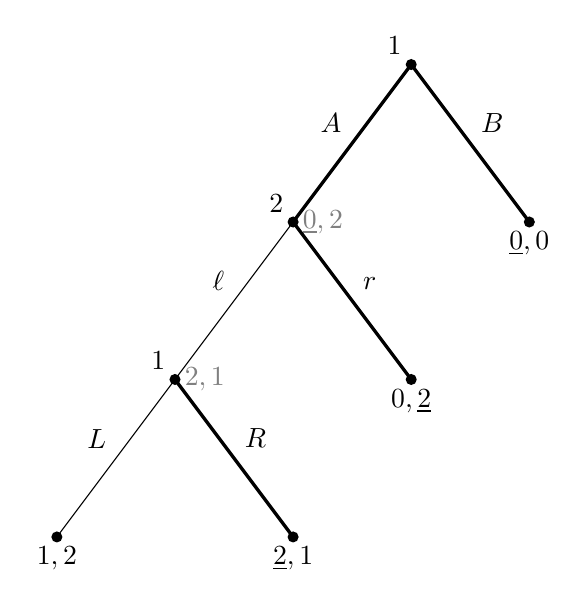
\begin{tikzpicture}
        \fill (0,0) circle (2pt) node [above left] {1};
        \fill (-1.5,-2) circle (2pt)
          node [above left] {2}
          node [right, gray] {$\underline{0},2$};
        \fill (1.5,-2) circle (2pt) node [below] {$\underline{0},0$};
        \fill (-3,-4) circle (2pt)
          node [above left] {1}
          node [right, gray] {$2,1$};
        \fill (0,-4) circle (2pt) node [below] {$0,\underline{2}$};
        \fill (-4.5,-6) circle (2pt) node [below] {$1,2$};
        \fill (-1.5,-6) circle (2pt) node [below] {$\underline{2},1$};

        \draw (-4.5,-6) -- (-3,-4) node [midway, above left] {$L$};
        \draw [very thick] (-3,-4) --  (-1.5,-6) node [midway, above right] {$R$};
        \draw (-1.5,-2) -- (-3,-4) node [midway, above left] {$\ell$};
        \draw [very thick] (-1.5,-2) -- (0,-4) node [midway, above right] {$r$};
        \draw [very thick] (-1.5,-2) -- (0,0) node [midway, above left] {$A$};
        \draw [very thick] (0,0) -- (1.5,-2) node [midway, above right] {$B$};
      \end{tikzpicture}
    \end{center}
    Damit ist $\text{SPNE} = \{(AR, r), (BR,r)\}$.
\end{enumerate}



\pagebreak

\listoftodos

\end{document} % chktex 17
